\documentclass[rgb,usenames,dvipsnames]{beamer}
\usepackage{linguex}
\usepackage{amssymb}
\usepackage{natbib}
\usepackage{stmaryrd}
\usepackage{cancel}
\usepackage{fontawesome}
\usepackage[most]{tcolorbox}
\usepackage{appendixnumberbeamer}

\expandafter\def\csname ver@etex.sty\endcsname{}
\usetheme{Konstanz}

\setcounter{secnumdepth}{3}
\format{169}

\usetikzlibrary{decorations.text,calc,arrows.meta}

\newcommand{\xmark}{\ding{55}}
\newcommand{\secref}[1]{{\S\ref{#1}}}
\newcommand{\emptyfill}{\hbox{}\hfill}
\newcommand{\boxright}{~\ensuremath{%
  \Box\kern-1.5pt
  \raise1pt\hbox{$\mathord{\rightarrow}$}}~}
\newcommand{\lrangle}[1]{\langle{#1}\rangle}
\newcommand{\entail}[2]{{#1}\Rightarrow{#2}}
\newcommand{\focus}[1]{{#1}$_F$}
\newcommand{\sem}[1]{\llbracket\text{#1}\rrbracket}
\newcommand{\type}[2]{\langle#1,#2\rangle}
\newcommand{\lambdac}[3]{[\lambda{#1}_{#2}.{#3}]}
\newcommand{\setof}[1]{\{#1\}} %
\newcommand{\tri}{\vartriangleleft}
\newcommand{\trieq}{\trianglelefteq}
\newcommand{\sqb}[1]{[#1]}
\newtcolorbox{myframe}[1][]{
  enhanced,
  arc=0pt,
  outer arc=0pt,
  colback=white,
  boxrule=0.8pt,
  #1
}
\makeatletter
\patchcmd{\NAT@test}{\else \NAT@nm}{\else \NAT@nmfmt{\NAT@nm}}{}{}
\DeclareRobustCommand\citepos
  {\begingroup
   \let\NAT@nmfmt\NAT@posfmt%
   \NAT@swafalse\let\NAT@ctype\z@\NAT@partrue
   \@ifstar{\NAT@fulltrue\NAT@citetp}{\NAT@fullfalse\NAT@citetp}}
\let\NAT@orig@nmfmt\NAT@nmfmt
\def\NAT@posfmt#1{\NAT@orig@nmfmt{#1's}}
\makeatother

\title{The Semantics and Pragmatics of Counterfactual Sentences at the Discourse Level}
\titleCorporateDesign{The Semantics and Pragmatics}{of Counterfactual Sentences at the}{Discourse Level: Sobel-Sequences and}{the Licensing of Negative Polarity Items}
\author{David Krassnig}
\date{22.05.2023}
\institute{University of Konstanz}

\begin{document}
\setmainfont{Arial}
\setsansfont{Arial}
\usebeamerfont{normalfont}
\begin{frame}[noframenumbering]
	\titlepage
\end{frame}
\setcounter{section}{-1}\section*{Dissertation Structure}

\begin{frame}[t]
    \sectionpage\vfill
    \begin{figure}
        \centering
        \begin{tikzpicture}
            \visible<1>{\node[inner sep=0pt] (russell) at (0,0) {
\includegraphics[width=.9\textwidth]{graphics/dissertationgraph-0.pdf}};}
            \visible<2>{\node[inner sep=0pt] (russell) at (0,0) {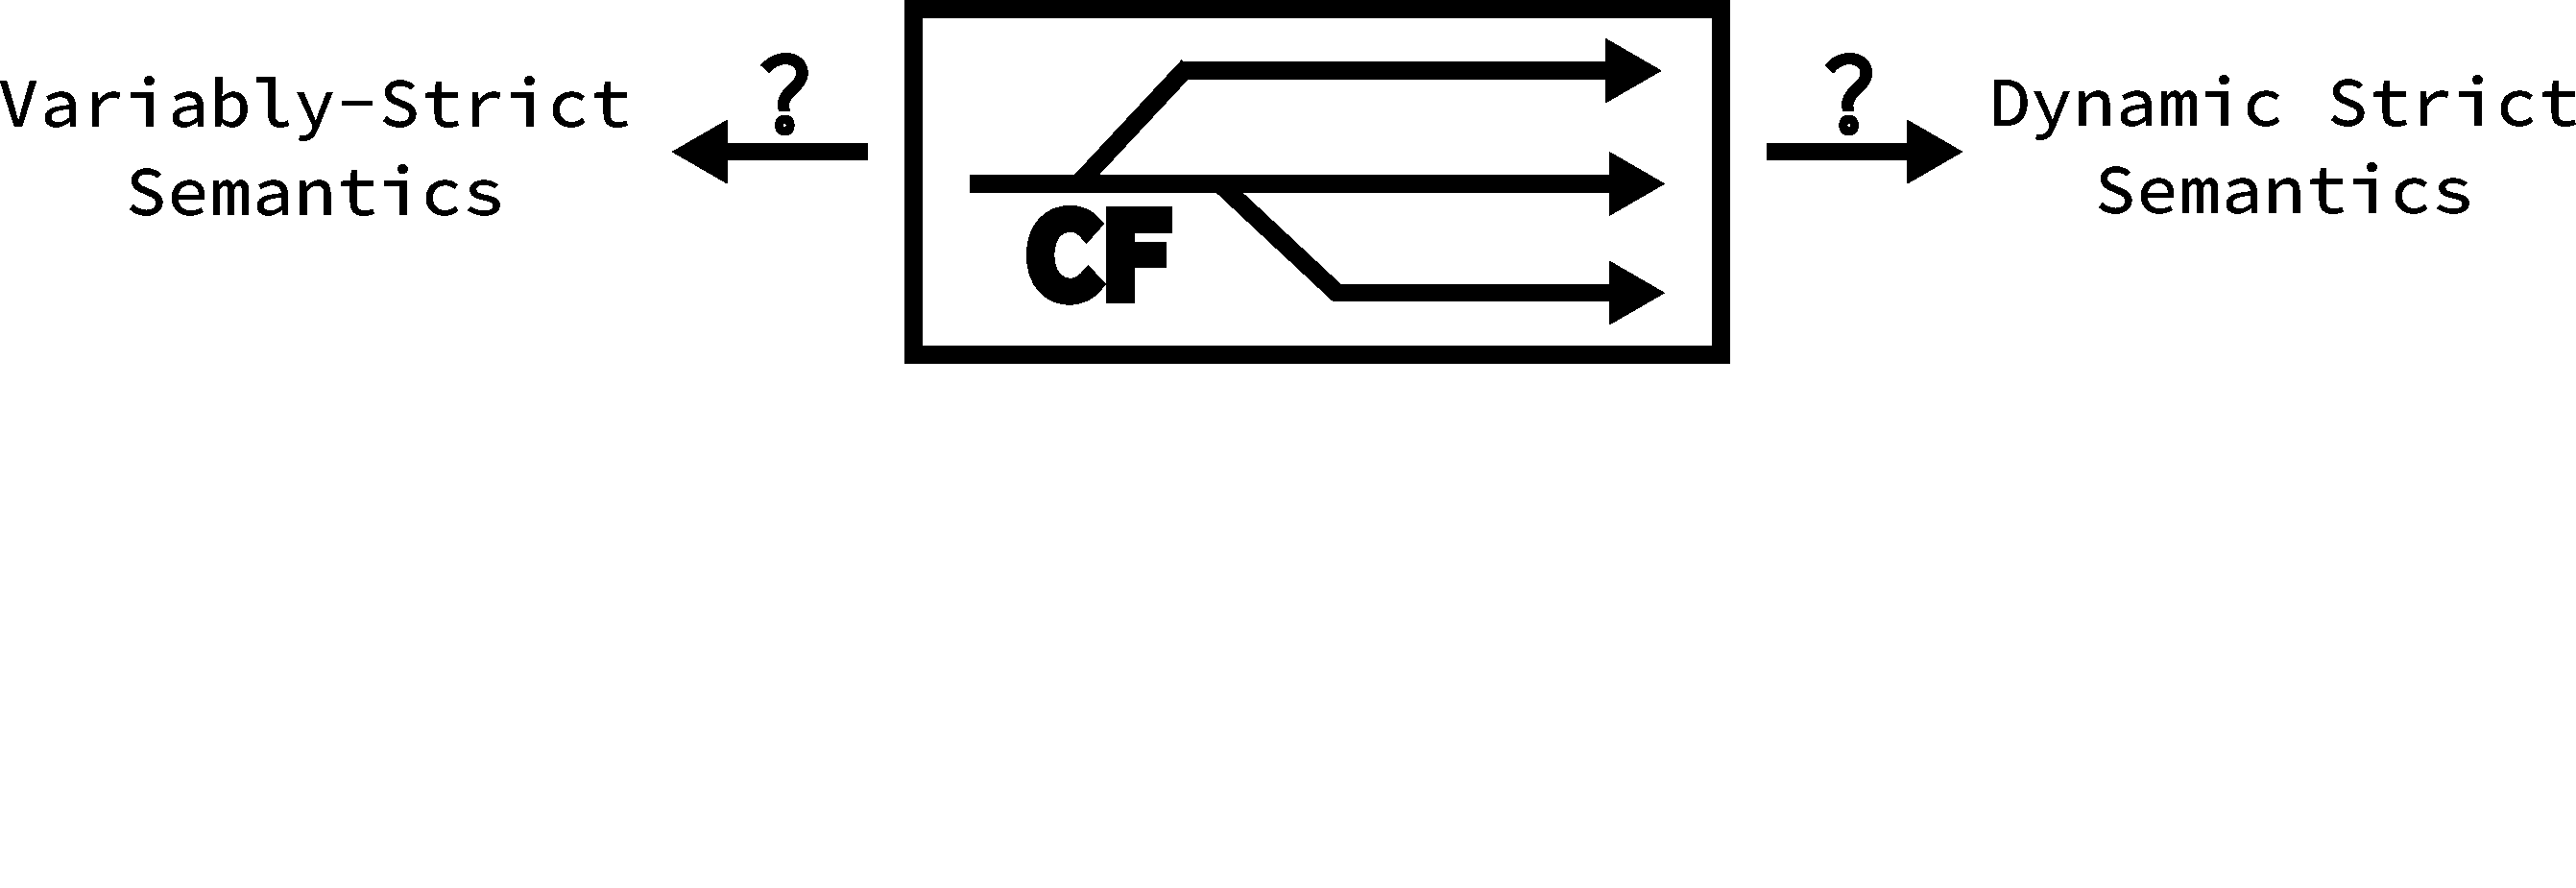
\includegraphics[width=.9\textwidth]{graphics/dissertationgraph-1.pdf}};}
            \visible<3>{\node[inner sep=0pt] (russell) at (0,0) {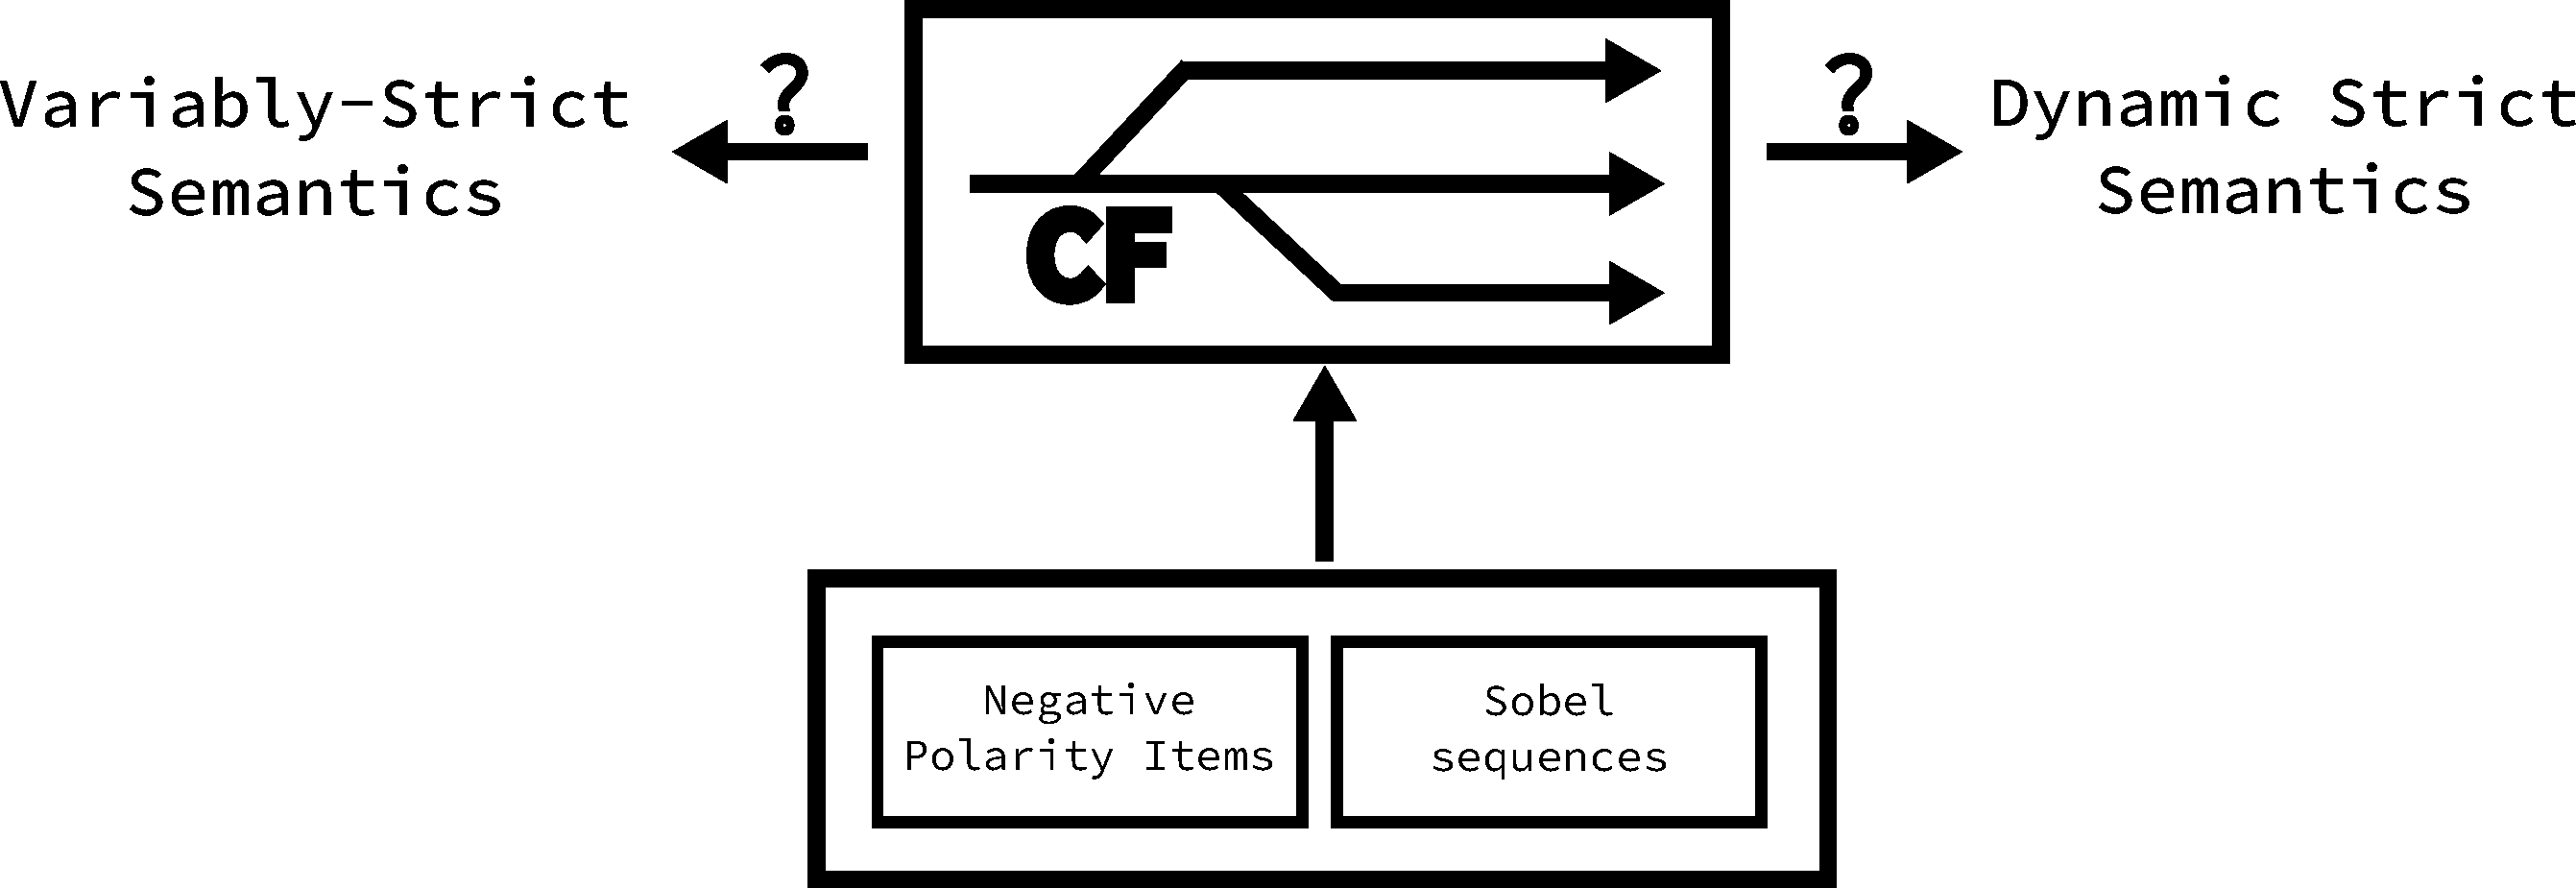
\includegraphics[width=.9\textwidth]{graphics/dissertationgraph-2.pdf}};}
            \visible<4>{\node[inner sep=0pt] (russell) at (0,0) {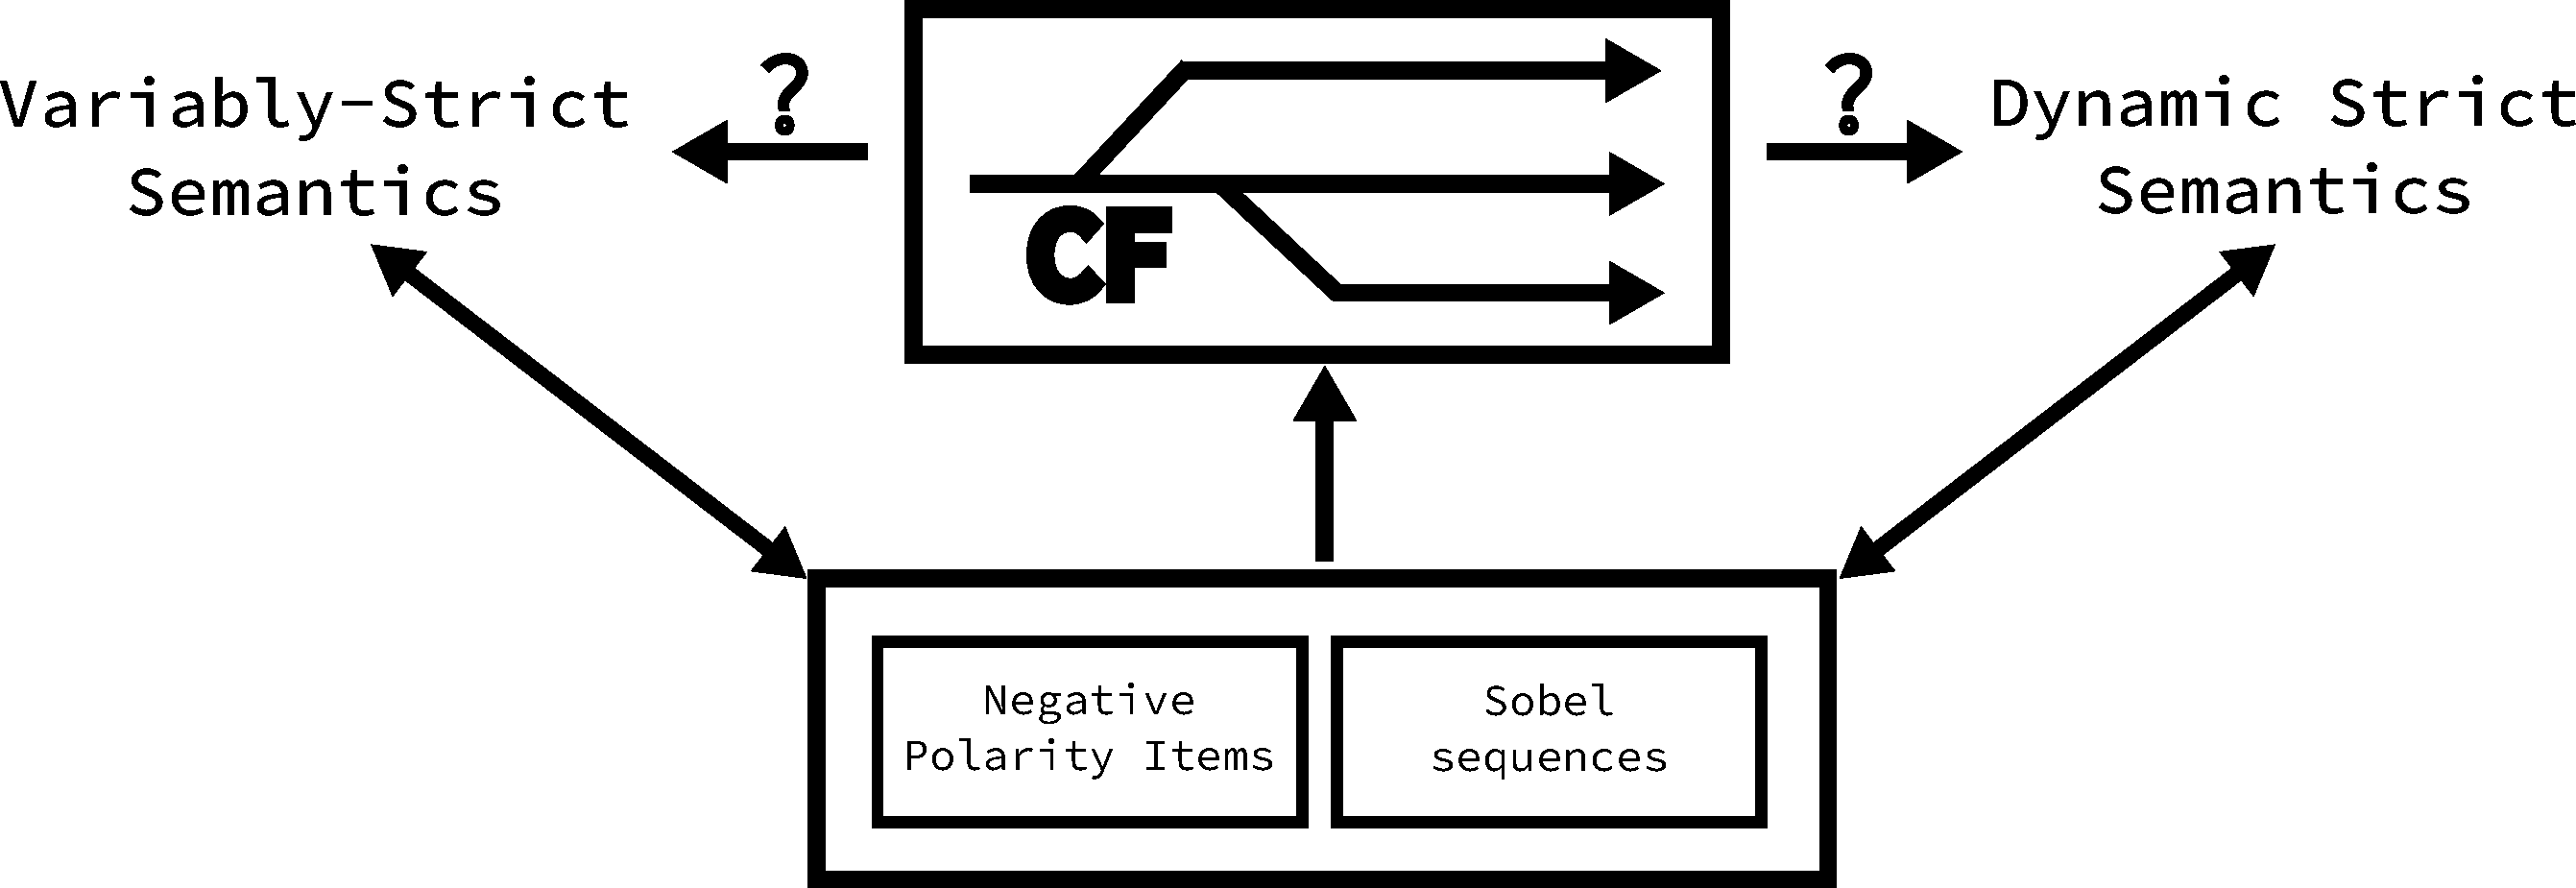
\includegraphics[width=.9\textwidth]{graphics/dissertationgraph-3.pdf}};}
        \end{tikzpicture}
    \end{figure}
    \vfill
\end{frame}

\begin{frame}[t]
	\sectionpage\vskip 9pt
	\begin{itemize}
	    %
		\item[$\blacksquare$]	\textbf{Chapter 2: Negative Polarity Items}\vskip 4.5pt
            \begin{itemize}
                \item<2-> Monotonicity-based approach vs \textit{even}-based approach\vskip 4.5pt
                \item<2-> \textit{Even-Based approach}: solved issue of negative polar question bias\vskip 4.5pt
                \item<2-> \textit{Even-Based approach}; better explanatory power for weak NPIs\vskip 9pt
            \end{itemize}
        \item[$\blacksquare$]	\textbf{Chapter 3: Negative Polarity Items in Conditional Antecedents}\vskip 4.5pt
            \begin{itemize}
                \item<3-> NPI distribution in conditional antecedents\vskip 4.5pt
                \item<3-> Interaction between \textit{even}-based approach and conditional semantics\vskip 4.5pt
                \item<3-> Dynamic strict Approach slightly superior to variably-strict approach
            \end{itemize}
	\end{itemize}
\end{frame}

\begin{frame}[t]
	\sectionpage\vskip 9pt
	\begin{itemize}
        \item[$\blacksquare$]	{\color<5->{seeblau100}\textbf{Chapter 4: Sobel Sequences -- Background and Empirical Data}}\vskip 4.5pt
            \begin{itemize}
                \item<2-> Established felicity distribution of reverse sequences (incl. via an experiment)\vskip 4.5pt
                \item<2-> Isolated felicity factors\vskip 9pt
            \end{itemize}
        \item[$\blacksquare$]	{\color<5->{seeblau100}\textbf{Chapter 5: A Contrast-Based Model of Reverse Sobel Sequence (In)Felicity}}\vskip 4.5pt
            \begin{itemize}
                \item<3-> Implemented model to derive felicity distribution of (reverse) Sobel sequences\vskip 4.5pt
                \item<3-> Showed its interaction with different conditional semantics\vskip 9pt
            \end{itemize}
        \item[$\blacksquare$]	\textbf{Chapter 6: Comparison of Our Model With Ippolito (2020)}\vskip 4.5pt
            \begin{itemize}
                \item<4-> Showed our model better accounts for known data\vskip 4.5pt
                \item<4-> Both models can be reconciled
            \end{itemize}
	\end{itemize}
\end{frame}
\begin{frame}[t]
	\frametitle{Table of Contents for Defence (Chapter 4 \&\ Chapter 5)}
    \setcounter{tocdepth}{1}
	\tableofcontents
\end{frame}
\section{Background Information}
\begin{frame}<2->[t]
\sectionpage\vskip 9pt

\begin{itemize}
    \item<1-> There are two competing approaches to model conditionals such as (1):
\end{itemize}\visible<2->{
\ex. $\color{seeblau100}\underbrace{\strut\strut\text{\phantom{tt}\color{black}If {\color{red}John went to the party\phantom{tt}}}\phantom\strut}_\text{\textbf{Antecedent}}\text{\color{black},}~\overbrace{\phantom{^t}\strut\text{\phantom{t}\color{OliveGreen}he would have fun\color{black}.\phantom{t}}\phantom{^t}}^\text{\textbf{Consequent}}$\label{ex:conditionals}

}\vskip 9pt
        \begin{itemize}
            \item<3-> Strict Analyses \citep{Peirce1896,Lewis1912,Lewis1914,Lewis1918,Fintel2001,Gillies2007}\vskip 9pt
                \begin{itemize}
                    \item<4-> Quantify over a single unstructured domain of accessible possible worlds
                \end{itemize}\vskip 18pt
            \item<3-> Variably-Strict Analyses \citep{Stalnaker1968,Lewis1973}\vskip 9pt
                \begin{itemize}
                    \item<5-> Quantify over differing possible world domains as determined by the antecedent 
                \end{itemize}
\end{itemize}
\end{frame}

\begin{frame}[t]
\sectionpage\vskip 9pt
\begin{itemize}
    \item<1-> What are (reverse) Sobel sequences?
\end{itemize}
\visible<2->{	\ex.	{\color{seeblau100}Sobel Sequence schematic}\\
	If $\color{red}\phi$ then $\color{OliveGreen}\chi$, but if $({\color{red}\phi}\land{\color{Orange}\psi})$ then not $\color{OliveGreen}\chi$\label{def:ss}

}	
\begin{itemize}
    \vskip 9pt
    \item<3-> Example Sobel sequence:\vspace{-6pt}
\end{itemize}
\visible<4->{    \ex.\textit{It is unlikely, but undecided whether John and Mary go to a small party. John dislikes Mary. Each decision is independent from and unknown to the other.}\\
    \textbf{$S_1$: }\phantom{\#}If {\color{red}John went to the party}, {\color{OliveGreen}he would have fun};\\\phantom{\textbf{$S_1$: }}\phantom{\#}but if {\color{red}John went to the party} and {\color{Orange}Mary went, too}, {\color{OliveGreen}he would} not {\color{OliveGreen}have fun}.

}\vskip 9pt
\begin{itemize}
    \item<5-> Generally felicitous
\end{itemize}
\end{frame}

\begin{frame}[t]
\sectionpage\vskip 9pt
\begin{itemize}
    \item<1-> What are (reverse) Sobel sequences?
\end{itemize}\vskip 9pt
\ref{def:ss}\hspace{14.5mm}{\color{seeblau100}Sobel Sequence schematic}~~~~~~~~~~~~~~~~/~~~{\color{seeblau100}Reverse Sobel Sequence schematic}\\
\phantom{\ref*{def:ss}}\hspace{14.5mm}If $\color{red}\phi$ then $\color{OliveGreen}\chi$, but if $({\color{red}\phi}\land{\color{Orange}\psi})$ then not $\color{OliveGreen}\chi$~~~/~~~If $({\color{red}\phi}\land{\color{Orange}\psi})$ then not $\color{OliveGreen}\chi$, but if $\color{red}\phi$ then $\color{OliveGreen}\chi$\vskip 9.25pt
\begin{itemize}
    \vskip 9pt
    \item<1-> Example reverse Sobel sequence:\vspace{-9.25pt}
\end{itemize}
\visible<2->{    \ex.\label{ex:badrss}\textit{It is unlikely, but undecided whether John and Mary go to a small party. John dislikes Mary. Each decision is independent from and unknown to the other.}\\
    \textbf{$S_1$: }\phantom{\#}If {\color{red}John went to the party} and {\color{Orange}Mary went, too}, {\color{OliveGreen}he would} not {\color{OliveGreen}have fun};\\\phantom{\textbf{$S_1$: }}\#but if {\color{red}John went to the party}, {\color{OliveGreen}he would have fun}.
    
}\vskip 9pt
\begin{itemize}
    \item<3-> Generally infelicitous \citep{Heim1994-MIT}
\end{itemize}
\end{frame}



\subsection{Variably-Strict Semantics}
\begin{frame}[t]
\subsectionpage\vskip 9pt
\ref{def:ss}\hspace{14.5mm}{\color{seeblau100}Sobel Sequence schematic}~~~~~~~~~~~~~~~~/~~~{\color{seeblau100}Reverse Sobel Sequence schematic}\\
\phantom{\ref*{def:ss}}\hspace{14.5mm}If $\color{red}\phi$ then $\color{OliveGreen}\chi$, but if $({\color{red}\phi}\land{\color{Orange}\psi})$ then not $\color{OliveGreen}\chi$~~~/~~~If $({\color{red}\phi}\land{\color{Orange}\psi})$ then not $\color{OliveGreen}\chi$, but if $\color{red}\phi$ then $\color{OliveGreen}\chi$\vskip 9.25pt\vskip 18pt
\begin{itemize}
            \item<1-> Variably-Strict Analyses \citep{Stalnaker1968,Lewis1973}
\end{itemize}\vskip 9pt
\visible<2->{\begin{myframe}[top=5pt,bottom=5pt,left=5pt,right=5pt,arc=5pt,auto outer arc]
{\begin{minipage}[h]{\textwidth}
\ex.	For all contexts $c$, `If $\color{red}\phi$ then $\color{OliveGreen}\chi$' is true at $w$ in $c$ iff \textbf{all the closest $\color{red}\phi$-worlds to $w$} are\linebreak\phantom{For all contexts $c$,} $\color{OliveGreen}\chi$-worlds, where closeness is determined by similarity.\label{def:variablystrict}

\end{minipage}}
\end{myframe}}\vskip 18pt
\begin{itemize}
    \item<3-> Similarity to evaluation world $w_0$ is reduced by each deviation from $w_0$ \citep{Lewis1973}
\end{itemize}
\end{frame}

\begin{frame}[t]
\subsectionpage\vskip 9pt
\begin{itemize}
    \item<1-> ${\color{red}\phi}\land{\color{Orange}\psi}$-worlds are one step ($\color{Orange}\psi$) in similarity further removed to $w_0$ than $\color{red}\phi$-worlds
\end{itemize}\vskip 9pt
\begin{figure}[ht!]
\centering
\begin{tikzpicture}
\visible<2->{
\coordinate (O) at (0,0);

	\draw[fill=white] (O) circle (2);
	\draw[fill=seeblau100] (O) circle (1.2);
	\draw[fill=white] (O) circle (0.4)node {w$_0$};

	\node at (0,0.7) {w$_1$};
	\node at (0.6,-0.5) {w$_2$};
	\node at (-0.6,-0.5) {w$_3$};
	
	\node at (0,-1.6) {w$_6$};
	\node at (-1,1.2) {w$_4$};
	\node at (1,1.2) {w$_5$};
	
	\node at (0,-2.5) {If $\color{red}\phi$, then $\color{OliveGreen}\chi$};

    \draw[color=seeblau100,line width=2mm,>={Triangle[length=4mm,width=4mm]},->] (2.5,0) -- (3.5,0);
 
	\begin{scope}[xshift=6cm]
		\coordinate (O) at (0,0);

	\draw[fill=seeblau100] (O) circle (2);
	\draw[fill=white] (O) circle (1.2);
	\draw[fill=white] (O) circle (0.4)node {w$_0$};

	\node at (0,0.7) {w$_1$};
	\node at (0.6,-0.5) {w$_2$};
	\node at (-0.6,-0.5) {w$_3$};
	
	\node at (0,-1.6) {w$_6$};
	\node at (-1,1.2) {w$_4$};
	\node at (1,1.2) {w$_5$};
	
	\node at (0,-2.5) {If ${\color{red}\phi}\land{\color{Orange}\psi}$, then not $\color{OliveGreen}\chi$};}\visible<3->{
	\node at (3,0) {\textbf{VS}};

	\begin{scope}[xshift=6cm]
		\coordinate (O) at (0,0);

	\draw[fill=seeblau100] (O) circle (2);
	\draw[fill=white] (O) circle (1.2);
	\draw[fill=white] (O) circle (0.4)node {w$_0$};

	\node at (0,0.7) {w$_1$};
	\node at (0.6,-0.5) {w$_2$};
	\node at (-0.6,-0.5) {w$_3$};
	
	\node at (0,-1.6) {w$_6$};
	\node at (-1,1.2) {w$_4$};
	\node at (1,1.2) {w$_5$};
	
	\node at (0,-2.5) {If ${\color{red}\phi}\land{\color{Orange}\psi}$, then not $\color{OliveGreen}\chi$};

    \draw[color=seeblau100,line width=2mm,>={Triangle[length=4mm,width=4mm]},->] (2.5,0) -- (3.5,0);
 
	\begin{scope}[xshift=6cm]
	\coordinate (O) at (0,0);

	\draw[fill=white] (O) circle (2);
	\draw[fill=seeblau100] (O) circle (1.2);
	\draw[fill=white] (O) circle (0.4)node {w$_0$};

	\node at (0,0.7) {w$_1$};
	\node at (0.6,-0.5) {w$_2$};
	\node at (-0.6,-0.5) {w$_3$};
	
	\node at (0,-1.6) {w$_6$};
	\node at (-1,1.2) {w$_4$};
	\node at (1,1.2) {w$_5$};
	
	\node at (0,-2.5) {If $\color{red}\phi$, then $\color{OliveGreen}\chi$};
	\end{scope}
	\end{scope}
	\end{scope}}
\end{tikzpicture}
\end{figure}
\begin{itemize}
    \item<4-> Either sequence type should be felicitous
\end{itemize}
\end{frame}


\subsection{(Semi)-Dynamic Strict Semantics}
\begin{frame}[t]
	\subsectionpage\vskip 9pt
	\begin{itemize}
		\item<1->	\citet{Fintel2001} \&~\citet{Gillies2007}
				\begin{itemize}
					\item<2->	Strict analysis 
					\item<3->   Added (semi-)dynamic component: \visible<4->{the \textit{Modal Horizon}}
					\end{itemize}
	\end{itemize}\vskip 9pt
\visible<5->{\begin{myframe}[top=5pt,bottom=5pt,left=5pt,right=5pt,arc=5pt,auto outer arc]{\begin{minipage}[h]{\textwidth}
	\ex.	For all contexts $c$, `If $\color{red}\phi$, then $\color{OliveGreen}\chi$' is true at $w$ in $c$ iff \textbf{all $\color{red}\phi$-worlds in a domain D}\linebreak\phantom{For all contexts $c$, }are $\color{OliveGreen}\chi$-worlds, where D is the modal horizon, which grows to\linebreak\phantom{For all contexts $c$, }encompass all worlds equal/greater in similarity to closest\linebreak\phantom{For all contexts $c$, }antecedent worlds if there is no antecedent world in D.\label{def:fintel}

\end{minipage}}\end{myframe}}\vskip 18pt
    \begin{itemize}
        \item<6-> Modal Horizon does not shrink easily~(requires effort)
    \end{itemize}
\end{frame}

\begin{frame}[t]
	\subsectionpage\vskip 9pt
	\begin{itemize}
        \item<1->	Conditional sequence affects modal horizon expansion
	\end{itemize}\vskip 9pt
	\begin{figure}[ht!]
\centering
\begin{tikzpicture}\visible<2->{
	\coordinate (O) at (0,0);

	\draw[fill=white] (O) circle (2);
	\draw[color=red,fill=seeblau100,line width=1mm] (O) circle (1.2);
	\draw[fill=white] (O) circle (0.4);

    \node at (0,0) {w$_0$};
	\node at (0,0.7) {w$_1$};
	\node at (0.6,-0.5) {w$_2$};
	\node at (-0.6,-0.5) {w$_3$};
	
	\node at (0,-1.6) {w$_6$};
	\node at (-1,1.2) {w$_4$};
	\node at (1,1.2) {w$_5$};
	
	\node at (0,-2.5) {If $\color{red}\phi$, then $\color{OliveGreen}\chi$};
	
	\draw[color=seeblau100,line width=2mm,>={Triangle[length=4mm,width=4mm]},->] (2.5,0) -- (3.5,0);
	
	\begin{scope}[xshift=6cm]
		\coordinate (O) at (0,0);

	\draw[color=red,fill=seeblau100,line width=1mm] (O) circle (2);
	\draw[fill=white] (O) circle (1.2);
	\draw[fill=white] (O) circle (0.4);

    \node at (0,0) {w$_0$};
	\node at (0,0.7) {w$_1$};
	\node at (0.6,-0.5) {w$_2$};
	\node at (-0.6,-0.5) {w$_3$};
	
	\node at (0,-1.6) {w$_6$};
	\node at (-1,1.2) {w$_4$};
	\node at (1,1.2) {w$_5$};
	
	\node at (0,-2.5) {If ${\color{red}\phi}\land{\color{Orange}\psi}$, then not $\color{OliveGreen}\chi$};}\visible<3->{
	\node at (3,0) {\textbf{VS}};
	
	\begin{scope}[xshift=6cm]
	\coordinate (O) at (0,0);

    \draw[color=red,line width=0.75mm] (O) circle (2.06);
	\draw[fill=seeblau100] (O) circle (2);
	\draw[fill=white] (O) circle (1.2);
	\draw[fill=white] (O) circle (0.4);

    \node at (0,0) {w$_0$};
	\node at (0,0.7) {w$_1$};
	\node at (0.6,-0.5) {w$_2$};
	\node at (-0.6,-0.5) {w$_3$};
	
	\node at (0,-1.6) {w$_6$};
	\node at (-1,1.2) {w$_4$};
	\node at (1,1.2) {w$_5$};
	
	\node at (0,-2.5) {If ${\color{red}\phi}\land{\color{Orange}\psi}$, then not $\color{OliveGreen}\chi$};
	
	\draw[color=seeblau100,line width=2mm,>={Triangle[length=4mm,width=4mm]},->] (2.5,0) -- (3.5,0);
	
	\begin{scope}[xshift=6cm]
		\coordinate (O) at (0,0);

	\draw[color=red,fill=seeblau100,line width=1mm] (O) circle (2);
	\draw[fill=seeblau100] (O) circle (1.2);
	\draw[fill=white] (O) circle (0.4);

	\node at (0,0) {w$_0$};
	\node at (0,0.7) {w$_1$};
	\node at (0.6,-0.5) {w$_2$};
	\node at (-0.6,-0.5) {w$_3$};
	
	\node at (0,-1.6) {w$_6$};
	\node at (-1,1.2) {w$_4$};
	\node at (1,1.2) {w$_5$};
	
	\node at (0,-2.5) {If $\color{red}\phi$, then $\color{OliveGreen}\chi$};
	\end{scope}
	\end{scope}
	\end{scope}}
\end{tikzpicture}
\label{fig:fintel}
\end{figure}
	\begin{itemize}
        \item<4->   Explains difference in felicity
	\end{itemize}
\end{frame}

\begin{frame}[t]
\sectionpage\vskip 9pt\textbf{\huge Current (to be updated) state:}\vskip 18pt
\begin{table}[]
    \centering
    \begin{tabular}{l||cc|ccc}
    Phenomenon  &    \multicolumn{2}{|c|}{Strict Semantics}    &  \multicolumn{3}{|c}{Variably-Strict Semantics}\\\hline\hline
                            &   \sout{Static}  & Dynamic    &   Basic    &     &    \\\hline
    \color{Gray}NPI Licensing           &   \sout{\color{Gray}Yes}     &  \color{Gray}Yes      &   \color{Gray}Partial   &      &   \\
    SS Felicity     &   \sout{No}      &  Yes      &   Yes     &        &   \\
    rSS Infelicity    &   \sout{Yes}      &   Yes      &   {No}     &        & 
    \end{tabular}
\end{table}
\end{frame}


\subsection{Variably-Strict Semantics Strike Back}
\begin{frame}[t]
	\sectionpage\vskip 9pt
	\ref{def:ss}\hspace{14.5mm}{\color{seeblau100}Sobel Sequence schematic}~~~~~~~~~~~~~~~~/~~~{\color{seeblau100}Reverse Sobel Sequence schematic}\\
\phantom{\ref*{def:ss}}\hspace{14.5mm}If $\color{red}\phi$ then $\color{OliveGreen}\chi$, but if $({\color{red}\phi}\land{\color{Orange}\psi})$ then not $\color{OliveGreen}\chi$~~~/~~~If $({\color{red}\phi}\land{\color{Orange}\psi})$ then not $\color{OliveGreen}\chi$, but if $\color{red}\phi$ then $\color{OliveGreen}\chi$\vskip 9.25pt\vskip 18pt
	\begin{itemize}
		\item   \citet{Moss2012} showed that some rSS are felicitous:
	\end{itemize}\vskip 18pt
	\visible<2->{\ex.	 \textit{(Holding up a dry match, with no water around)} If {\color{red}I had struck this match} and {\color{Orange}it had been soaked}, {\color{OliveGreen}it would} not {\color{OliveGreen}have lit}. But if {\color{red}I \MakeUppercase{had} struck this match}, {\color{OliveGreen}it would have lit}.\\%
	\vspace{-5mm}\emptyfill(adapted from \citet[p. 106]{Stalnaker1968} by \citet[p. 487]{Lewis2017})\label{ex:match}%

}
\end{frame}

\begin{frame}[t]
\sectionpage\vskip 9pt\textbf{\huge Current State:}\vskip 18pt
\begin{table}[]
    \centering
    \begin{tabular}{l||cc|ccc}
    Phenomenon  &    \multicolumn{2}{|c|}{Strict Semantics}    &  \multicolumn{3}{|c}{Variably-Strict Semantics}\\\hline\hline
                            &   \sout{Static}  & Dynamic    &   Basic    &     &    \\\hline
    \color{Gray}NPI Licensing           &   \sout{\color{Gray}Yes}     &  \color{Gray}Yes      &   \color{Gray}Partial   &      &   \\
    SS Felicity     &   \sout{No}      &  Yes      &   Yes     &        &   \\
    rSS Infelicity    &   \sout{Yes}      &   Yes      &   {No}     &        & \\
    \textbf{rSS Felicity}    &   \sout{\textbf{No}}  &   \textbf{No}  &   \textbf{Yes} & 
    \end{tabular}
\end{table}
\end{frame}

\begin{frame}[t]
\subsectionpage\vskip 9pt
\begin{itemize}
	\item<1->	Dynamic strict analyses and variably-strict analyses on equal footing\vskip 18pt
	\item<1->   Unable to account for felicity/infelicity of reverse Sobel sequences:\vskip 18pt
\end{itemize}\visible<2->{
\begin{minipage}[h]{0.25\linewidth}
\begin{table}[h]
    \begin{tabular}{l||c}
                &   Felicity\\\hline\hline
          SS    &   \checkmark\\
          rSS   &   \checkmark,~\#
    \end{tabular}
\end{table}
\begin{tikzpicture}[overlay]
\visible<3->{\draw[red, line width=2pt] (3.5,0.75) ellipse (1cm and 0.4cm);}
\visible<4->{\node (fig1) at (4.4,0.275) {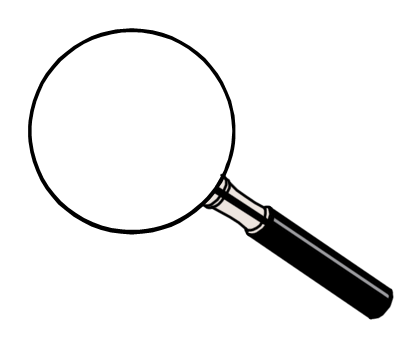
\includegraphics[scale=0.33]{graphics/glass.png}};}
\end{tikzpicture} 
\end{minipage}}\hspace{1cm}\visible<4->{
\begin{minipage}{0.6\linewidth}
\textbf{What is the deciding factor?}

\end{minipage}}
\end{frame}
\section{Felicity Distribution and Felicity Factors}
\begin{frame}[t]
\sectionpage\vskip 18pt
\begin{itemize}
    \item<1->	Researchers posited several possible factors that influence rSS felicity:\vskip 18pt
			\begin{itemize}
                \item<1->	{{Degree of World Dissimilarity between ${\color{red}\phi}$ and ${\color{Orange}\psi}$}} \citep{Lewis2017,Krassnig2017}\vskip 18pt
                \item<2->   Contrastive Stress in the second antecedent \citep{Klecha2014a,krassnig2022ReverseSobel}\vskip 9pt
				\item<3->	{Causal links between ${\color{red}\phi}$ and ${\color{Orange}\psi}$} \citep{Klecha2014a}\vskip 9pt
                \item<4->   Counterfactuality of ${\color{red}\phi}$ and ${\color{Orange}\psi}$ \citep{krassnig2022ReverseSobel}\vskip 9pt
				\item<5->	{Epistemic irresponsibility of considering ${\color{red}\phi}$ without ${\color{Orange}\psi}$} \citep{Moss2012}
			\end{itemize}
\end{itemize}
\end{frame}

\subsection{Dynamic World Orderings and Relevance}
\begin{frame}[t]
\subsectionpage\vskip 9pt%
\begin{itemize}
    \item \citet{Lewis2017} proposed the following factor:\vskip 9pt
        \begin{itemize}
            \item<2-> rSS with dissimilar antecedent world sets are felicitous
            \item<3-> rSS with similar antecedent world sets are infelicitous
        \end{itemize}
\end{itemize}\vskip 18pt
\visible<4->{
\begin{minipage}[h]{0.55\linewidth}
\begin{table}[h]
    \begin{tabular}{l||c|c}
                &   Dissimilar     &   Similar\\\hline\hline
          SS    &   \checkmark  &   \checkmark\\
          rSS   &   \checkmark  &   \#
    \end{tabular}
\end{table}
\end{minipage}}\vskip 9pt
\begin{itemize}
    \item<5-> Tough to verify via informal native speaker judgements
    \item<6-> No experimental work on rSS so far\vskip 9pt
    \item<7-> So, we conducted an experiment to test \citepos{Lewis2017} predictions
\end{itemize}
    
\end{frame}

\subsubsection{Experiment}
\begin{frame}<3->[t]
\subsectionpage
	
	\textbf{Empirical Testing of \citet{Lewis2017}}\vskip 9pt
    \begin{itemize}
        \item<3-> Participants (n=41 after excl.) were asked to rate target items on a scale from 1 to 5\vskip 9pt
            \begin{itemize}
                \item<4-> 1 = Sounds very natural
                \item<4-> 5 = Sounds very unnatural
            \end{itemize}\vskip 9pt
        \item<5-> Four target conditions
            \begin{itemize}
                \item<6-> Control (SS \& other felicitous conditional sequences)
                \item<7-> Similar (non-counterfactual rSS where ${\color{red}\phi}\land{\color{Orange}\psi}$ and $\color{red}\phi$ are similar by context)
                \item<7-> Dissimilar (non-counterfactual rSS where ${\color{red}\phi}\land{\color{Orange}\psi}$ and $\color{red}\phi$ are dissimilar by context)
                \item<8-> Disjoint (rSS where ${\color{red}\phi}\land{\color{Orange}\psi}$ was counterfactual%
                )
            \end{itemize}\vskip 9pt
        \item<9-> All items were acausal by nature and indicated contrastive stress
    \end{itemize}
\end{frame}

\begin{frame}[t]
    \subsectionpage\visible<3->{
    \begin{minipage}{0.425\linewidth}
    \begin{figure}[ht!]
    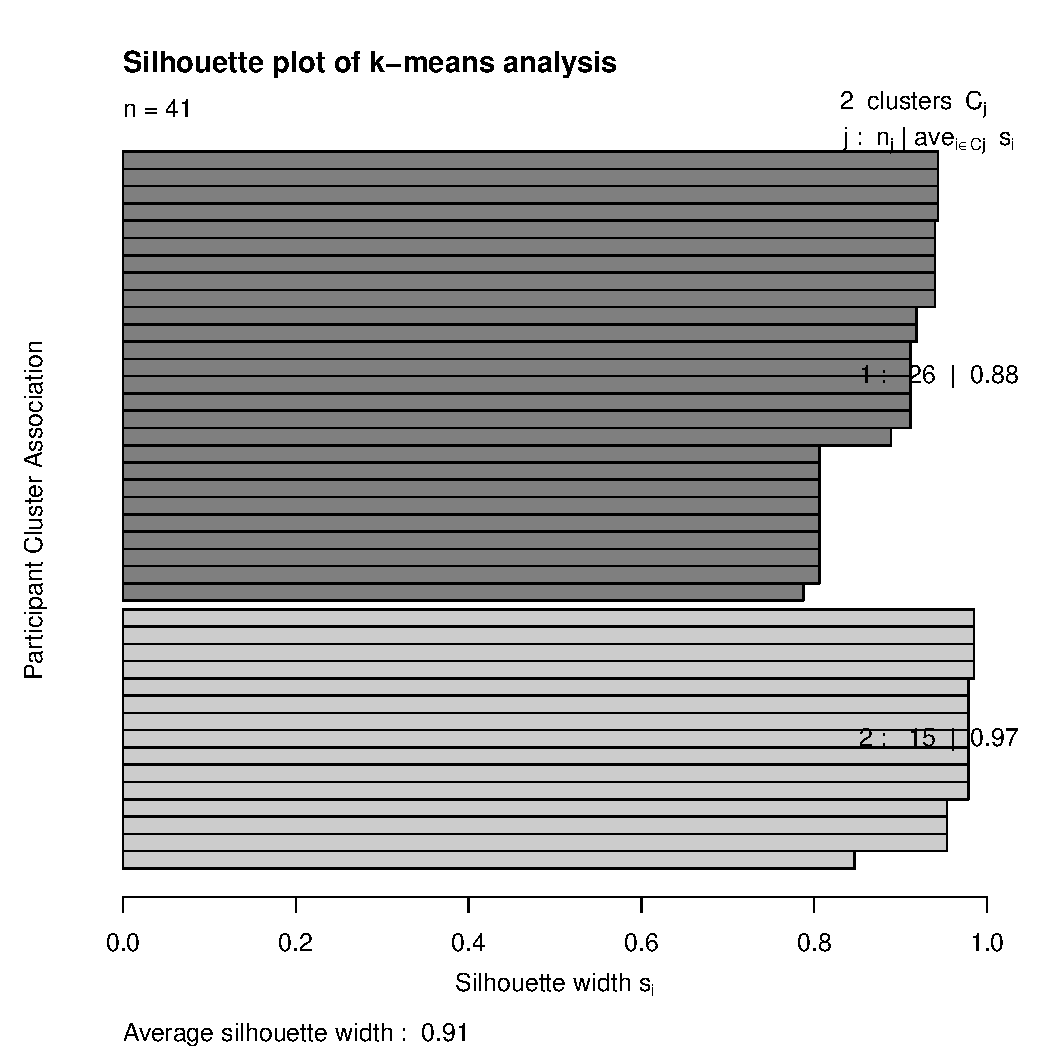
\includegraphics[width=\linewidth,page=1,trim=0pt 30pt 0pt 30pt]{graphics/silhouette.pdf}
\end{figure}
\end{minipage}}%
\begin{minipage}[t]{0.575\linewidth}\vspace*{-40mm}
    \begin{itemize}
        \item<1-> Dissimilar condition results seemed polarising\vskip 9pt
        \item<2-> Conducted a k-means analysis on results\vskip 9pt
        \item<4-> Two clusters with very high average confidence
    \end{itemize}
\end{minipage}
\end{frame}

\begin{frame}[t]
    \subsectionpage\vskip 7.5pt
    \hspace*{45mm}\textbf{Cluster 1}\hspace{72.5mm}\textbf{Cluster 2}\vspace{-7.5mm}
    \begin{figure}[ht!]
\begin{minipage}{0.9\linewidth}
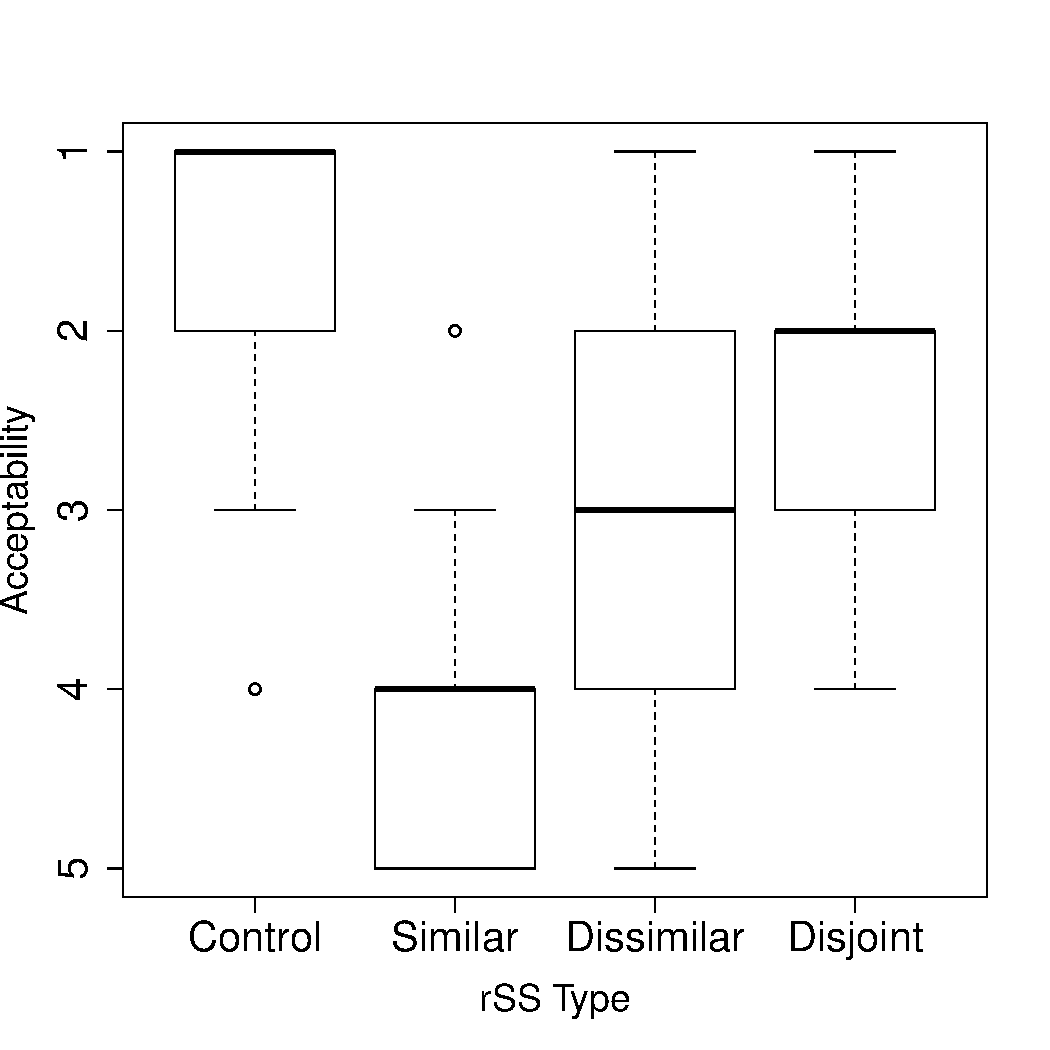
\includegraphics[width=0.425\linewidth,page=1]{graphics/boxplots.pdf}\hspace{10mm}
\includegraphics[width=0.425\linewidth,page=2]{graphics/boxplots.pdf}
\end{minipage}%
\end{figure}
\end{frame}

\begin{frame}[t]
\subsectionpage\vskip 9pt
\begin{itemize}
    \item<1-> No significant difference between clusters except dissimilar rSS condition\vskip 9pt
        \begin{itemize}
            \item<1-> First cluster: Acceptability judgements go haywire\vskip 9pt
        \end{itemize}
    \item<1-> Both clusters: Counterfactual/Disjoint condition almost perfect\vskip 9pt
    \item<1-> Second cluster: No significant difference between dissimilar and similar condition\vskip 18pt
    \item<2-> We therefore reject \citepos{Lewis2017} hypothesis\vskip 9pt
    \item<3-> Dissimilarity does not reliably increase the odds of felicity
\end{itemize}
\end{frame}

\begin{frame}[t]
\subsectionpage\vskip 9pt
\begin{itemize}
    \item<1->	Researchers posited several possible factors that influence rSS felicity:\vskip 18pt
			\begin{itemize}
                \item<1->	{\sout{Degree of World Dissimilarity between ${\color{red}\phi}$ and ${\color{Orange}\psi}$}} \citep{Lewis2017,Krassnig2017}\vskip 18pt
                \item<1->   Contrastive Stress in the second antecedent \citep{Klecha2014a,krassnig2022ReverseSobel}\vskip 9pt
				\item<1->	{Causal links between ${\color{red}\phi}$ and ${\color{Orange}\psi}$} \citep{Klecha2014a}\vskip 9pt
                \item<1->   Counterfactuality of ${\color{red}\phi}$ and ${\color{Orange}\psi}$ \citep{krassnig2022ReverseSobel}\vskip 9pt
				\item<1->	{Epistemic irresponsibility of considering ${\color{red}\phi}$ without ${\color{Orange}\psi}$} \citep{Moss2012}
			\end{itemize}
\end{itemize}
\end{frame}

\subsection{Contrastive Stress}
\begin{frame}[t]
    \subsectionpage\vskip 9pt
    \begin{itemize}
        \item<1-> \citet{Klecha2014a}: Some overtly different lexical item must be contrastively stressed\vskip 9pt
        \item<2-> \citet{krassnig2022ReverseSobel}: Auxiliary verbs may be contrastively stressed instead\vskip 9pt
        \item<3-> Without any kind of contrastive stress, rSS are infelicitous
    \end{itemize}\vskip 9pt
    \visible<4->{
    	\ex.[\ref{ex:match}]	 \label{ex:contrastaux-good}\textit{(Holding up a dry match, with no water around)} If {\color{red}I had struck this match} and {\color{Orange}it had been soaked}, {\color{OliveGreen}it would} not {\color{OliveGreen}have lit}. But if {\color{red}I \MakeUppercase{had} struck this match}, {\color{OliveGreen}it would have lit}.
    
    }
    \visible<5->{
    	\ex.\label{ex:contrastaux-bad}\textit{(Holding up a dry match, with no water around)} If {\color{red}I had struck this match} and {\color{Orange}it had been soaked}, {\color{OliveGreen}it would} not {\color{OliveGreen}have lit}. \#But if {\color{red}I{'d} struck this match}, {\color{OliveGreen}it would have lit}.
    
    }\vskip 9pt
    \begin{itemize}
        \item<6-> We take the presence of contrastive stress for granted for all future factors
    \end{itemize}
\end{frame}

\subsection{Causality}
\begin{frame}[t]
    \subsectionpage\vskip 9pt
    \begin{itemize}
        \item<1-> \citet{Klecha2014a}: another factor is causality\vskip 9pt
            \begin{itemize}
                \item<2-> If ${\color{red}\phi}$ precedes ${\color{Orange}\psi}$ on some causal chain, then the rSS is infelicitous
            \end{itemize}\vskip 18pt
        \item<3-> \textbf{Acausal rSS}~~~($\color{red}\phi$ does not causally precede $\color{Orange}\psi$)
        \end{itemize}
 \visible<4->{
    	\ex.[\ref{ex:match}]	 \label{ex:acausaloki}\textit{(Holding up a dry match, with no water around)} If {\color{red}I had struck this match} and {\color{Orange}it had been soaked}, {\color{OliveGreen}it would} not {\color{OliveGreen}have lit}. But if {\color{red}I \MakeUppercase{had} struck this match}, {\color{OliveGreen}it would have lit}.%
    
    }
    \vskip 18pt
    \begin{itemize}
        \item<5-> \textbf{Causal rSS}~~~($\color{red}\phi$ causally precedes $\color{Orange}\psi$)
    \end{itemize}
    \visible<6->{
    \ex.\label{ex:causalnoki}\textit{(Holding up a dry match, with no water around)} If {\color{red}I had struck this match} and {\color{Orange}it had snapped}, {\color{OliveGreen}it would} not {\color{OliveGreen}have lit}. \#But if {\color{red}I \MakeUppercase{had} struck this match}, {\color{OliveGreen}it would have lit}.
    
    }
\end{frame}

\subsection{Counterfactuality}
\begin{frame}[t]
    \subsectionpage\vskip 9pt
    \begin{itemize}
        \item<1-> \citet{krassnig2022ReverseSobel}: Non-Counterfactuality has exact same impact as causality\vskip 9pt
            \begin{itemize}
                \item<2-> If $\color{red}\phi$ and ${\color{Orange}\psi}$ are non-counterfactual, then the rSS is infelicitous
            \end{itemize}\vskip 18pt
        \item<3-> \textbf{Counterfactual Acausal rSS}~~~($\color{red}\phi$ and $\color{Orange}\psi$ are counterfactual)
        \end{itemize}
    \visible<4->{
    	\ex.[\ref{ex:match}]	 \label{ex:rss-cf-good}\textit{(Holding up a dry match, with no water around)} If {\color{red}I had struck this match} and {\color{Orange}it had been soaked}, {\color{OliveGreen}it would} not {\color{OliveGreen}have lit}. But if {\color{red}I \MakeUppercase{had} struck this match}, {\color{OliveGreen}it would have lit}.
    
    }\vskip 18pt
    \begin{itemize}
        \item<5-> \textbf{Non-Counterfactual Acausal rSS}~~~($\color{red}\phi$ and $\color{Orange}\psi$ are non-counterfactual)
    \end{itemize}
    \visible<6->{
    	\ex.\label{ex:rss-ncf-bad}\textit{(Holding up a dry match)} If {\color{red}I struck this match tomorrow} and {\color{Orange}it was soaked}, {\color{OliveGreen}it would} not {\color{OliveGreen} light}. \#But if {\color{red}I \MakeUppercase{were} to strike this match tomorrow}, {\color{OliveGreen}it would light}.
    
    }
\end{frame}

\subsection{Epistemic Dismissal}
\begin{frame}[t]
    \subsectionpage
    \begin{itemize}
        \item<1-> \citet{Moss2012}: If {\color{Orange}$\psi$} is (responsibly) epistemically dismissed, the rSS is felicitous\vskip 6pt
        \item<2-> \citet{krassnig2022ReverseSobel}: Epistemic dismissal of {\color{Orange}$\psi$} rescues any contrastively stressed rSS\vskip 14pt
        \item<3-> \textbf{Epistemically Undismissed Non-Counterfactual Causal rSS}~~~($\color{Orange}\psi$ is undismissed)
    \end{itemize}
    \visible<4->{
    	\ex.\label{ex:rss-no-exclusion}\textit{(Holding up a dry match)} If {\color{red}I struck this match tomorrow} and {\color{Orange}it snapped}, {\color{OliveGreen}it would} not {\color{OliveGreen} light}. \#But if {\color{red}I \MakeUppercase{were} to strike this match tomorrow}, {\color{OliveGreen}it would light}.
    
    }\vskip 14pt
    \begin{itemize}
        \item<5-> \textbf{Epistemically Dismissed Non-Counterfactual Causal rSS}~~~($\color{Orange}\psi$ is dismissed)
    \end{itemize}
    \visible<6->{
    	\ex.\label{ex:rss-exclusion}\textit{(Holding up a dry match)} If {\color{red}I struck this match tomorrow} and {\color{Orange}it snapped}, {\color{OliveGreen}it would} not {\color{OliveGreen} light}. But we all know that I'm the national champion at match striking and never snap a match. So, if {\color{red}I \MakeUppercase{were} to strike this match tomorrow}, {\color{OliveGreen}it would light}.
    
    }
\end{frame}

\begin{frame}[t]
    \subsectionpage
    \begin{itemize}
        \item<1-> This dismissal may also be covert via context\vskip 18pt
        \item<2-> \textbf{Epistemically Dismissed Non-Counterfactual Causal rSS}~~~($\color{Orange}\psi$ is dismissed)
    \end{itemize}
    \visible<2->{
    	\ex.\label{ex:rss-exclusion-covert}\textit{(The speaker knows that Mary would never agree to marry John, which is unbeknownst to the other discourse participant.)} Well, let me put it like this: If {\color{red}John proposed to Mary tomorrow} and {\color{Orange}she said yes}, {\color{OliveGreen}he would be very happy}. But if {\color{red}John \MakeUppercase{were} to propose to Mary tomorrow}, {\color{OliveGreen}he would} not {\color{OliveGreen} be happy at all}.
    
    }
\end{frame}

\subsection*{Summary}
\begin{frame}[t]
\subsectionpage\vskip 9pt
\begin{itemize}
    \item<1-> Contrastive stress allows for rSS felicity\vskip 9pt
    \item<2-> Causality and Non-Counterfactuality render rSS infelicitous\vskip 9pt
    \item<3-> Epistemic dismissal of {\color{Orange}$\psi$} rescues all contrastively stressed rSS
\end{itemize}\vskip 18pt
\visible<4->{
\begin{minipage}[h]{0.9\linewidth}
\begin{table}[h]
\caption{Felicity distribution, presupposing the presence of contrastive stress}\vskip -18pt
\resizebox{\textwidth}{!}{%
    \begin{tabular}{l||c|c|c|c|c|c|c}
                &   \multicolumn{3}{|c|}{Acausal}     &  \multicolumn{3}{|c}{Causal}\\\hline
                & CF  &   \multicolumn{2}{|c|}{Non-CF}    & \multicolumn{2}{|c|}{CF}  &   \multicolumn{2}{|c}{Non-CF}\\\hline
                &   & Undismissed & Dismissed   &  Undismissed & Dismissed & Undismissed & Dismissed\\\hline\hline
          SS    &   \checkmark  &   \checkmark  &   N/A  &   \checkmark    &   N/A  &   \checkmark & N/A\\
          rSS   &   \checkmark\ref{ex:match}  &   \#\ref{ex:rss-ncf-bad}  &   \checkmark  &   \#\ref{ex:causalnoki}  & \checkmark &   \#\ref{ex:rss-no-exclusion}    &   \checkmark\ref{ex:rss-exclusion}
    \end{tabular}}
\end{table}
\end{minipage}}
    
\end{frame}

\section{Implementation}
\begin{frame}[t]
\sectionpage\vskip 18pt
    \begin{itemize}
        \item<1-> Questions to be answered:\vskip 18pt
            \begin{enumerate}
                \item<2-> Why are rSS without contrastive stress infelicitous?\vskip 9pt
                \item<2-> How does contrastive stress help?\vskip 9pt
                \item<2-> Why contrastive stress on auxiliary verb?\vskip 9pt
                \item<3-> How does a causal link between {\color{red}$\phi$} and {\color{Orange}$\psi$} cause infelicity?\vskip 9pt
                \item<3-> How does non-counterfactuality cause infelicity?\vskip 9pt
                \item<4-> How does the epistemic dismissal of {\color{Orange}$\psi$} rescue rSS?
            \end{enumerate}
	\end{itemize}
\end{frame}

\subsection{Why are rSS without contrastive stress infelicitous?}
\begin{frame}[t]
    \subsectionpage\vskip 9pt
    \begin{itemize}
        \item<1-> rSS without contrastive stress are routinely infelicitous\vskip 9pt
        \item<2-> Requirement: Some ingredient renders rSS infelicitous without further intervention\vskip 4.5pt
            \begin{itemize}
                \item<3-> Infelicity via contradiction: Extend {\color{Orange}$\psi$} into the {\color{red}$\phi$}-conditional
                \item<4-> Dynamic Strict Semantics: Expanding Modal Horizon
                \item<5-> Variably-Strict Semantics: Modal Subordination \citep{Klecha2014a}
            \end{itemize}\vskip 18pt
        \item<6-> Modal Subordination: interpret current sentence as subordinate to preceding modal\vskip 4.5pt
            \begin{itemize}
                \item<7-> Second consequent interpreted w.r.t. both its and the preceding antecedent
            \end{itemize}
    \end{itemize}
    \visible<8->{\ex. \resizebox{576pt}{!}{If $({\color{red}\phi}\land{\color{Orange}\psi})$ then not $\color{OliveGreen}\chi$; but if $\color{red}\phi$ then $\color{OliveGreen}\chi$ $\Rightarrow$ If $({\color{red}\phi}\land{\color{Orange}\psi})$ then not $\color{OliveGreen}\chi$; but if $({\color{red}\phi}\land{\color{Orange}\psi})\land\color{red}\phi$ then $\color{OliveGreen}\chi$}\\%
    \hspace{-0.75mm}\resizebox{576pt}{!}{\phantom{If $({\color{red}\phi}\land{\color{Orange}\psi})$ then not $\color{OliveGreen}\chi$; but if $\color{red}\phi$ then $\color{OliveGreen}\chi$ }$\Rightarrow$ If $({\color{red}\phi}\land{\color{Orange}\psi})$ then not $\color{OliveGreen}\chi$; but if $({\color{red}\phi}\land{\color{Orange}\psi})\phantom{\land\color{red}\phi}$ then $\color{OliveGreen}\chi$}

    }
\end{frame}

\subsection{How does contrastive stress help?}
\begin{frame}[t]
    \subsectionpage\vskip 9pt
    \begin{itemize}
        \item<2-> Our proposal: contrastive topic\vskip 4.5pt
        \begin{itemize}
            \item<3-> Establish two topics as logically disjoint and independent
        \end{itemize}
    \end{itemize}
    \visible<4->{\ex. a. What do your siblings do?\\
         b. \textbf{{\color{seeblau100!75!black}[My [SIster]\textsubscript{Focus}]\textsubscript{Topic}}} [studies MEDicine]\textsubscript{Focus}, and \textbf{{\color{seeblau100!75!black}[my [BROther]\textsubscript{Focus}]\textsubscript{Topic}}} is\\\phantom{b. }[working on a FREIGHT ship]\textsubscript{Focus}.\hfill\citep[p.~44]{Krifka2007}

}
    \visible<5->{\ex. a. What do your siblings do?\\
         b. \textbf{{\color{seeblau100!75!black}[My [BROthers]\textsubscript{Focus}]\textsubscript{Topic}}} [study MEDicine]\textsubscript{Focus}, and \#\textbf{{\color{seeblau100!75!black}[my [LITtle}}\\ \phantom{b. }\textbf{{\color{seeblau100!75!black}brother]\textsubscript{Focus}]\textsubscript{Topic}}} is [working on a FREIGHT ship]\textsubscript{Focus}.\hfill\citep[p.~267]{Krifka2007}\vskip 18pt

}
    \begin{itemize}
        \item<6-> Conditional antecedents set aboutness topic \citep{Ebert2008,Ebert2014}\vskip 4.5pt
        \item<7-> Contrastive topic gives impetus to interpret ${\color{red}\phi}$-conditional logically on its own
    \end{itemize}
\end{frame}

\subsection{Why contrastive stress on the auxiliary verb?}
\begin{frame}[t]
    \subsectionpage\vskip 9pt
    \begin{itemize}
        \item<2-> How are the auxiliary verbs semantically disjoint?\vskip 9pt
        \item<3-> Our proposal: actual target is tense-aspect-mood (TAM) morphology\vskip 4.5pt
            \begin{itemize}
                \item<4-> Antecedental TAM morphology connected to conditional's world variable
                \item<5-> TAM treated as type of bound pro-world \citep{Schlenker2005}
                \item<6-> Contrastively stressed pro-worlds behave like contrastively stressed pronouns
            \end{itemize}\vskip 4.5pt
        \item<7-> How do contrastively stressed pronouns behave?\vskip 4.5pt
            \begin{itemize}
                \item<8-> Only felicitous if the binders' domains are disjoint \citep{Sauerland1998,Sauerland1999} 
            \end{itemize}
    \end{itemize}
    \visible<9->{\ex. \resizebox{576pt}{!}{Every fourth grade boy\textsubscript{i} called {\color{seeblau100!75!black}his\textsubscript{i}} mother, but no FIFTH grade boy\textsubscript{j} called {\color{seeblau100!75!black}HIS\textsubscript{j}} mother.}

}
    \visible<10->{\ex. \resizebox{576pt}{!}{I wanted every student\textsubscript{i} to call {\color{seeblau100!75!black}his\textsubscript{i}} father, \#but only every YOUNG student\textsubscript{j} called {\color{seeblau100!75!black}HIS\textsubscript{j}} father.}

}
\end{frame}

\begin{frame}[t]
    \subsectionpage\vskip 9pt
    \begin{itemize}
        \item<1-> Formal model of this by \citet{Jacobson2004}:\vskip 4.5pt
            \begin{itemize}
                \item<2-> Bound pronoun: a partial identity function (range: its binder's domain)
            \end{itemize}
    \end{itemize}
    \visible<3->{\ex.  a. $\sem{his\textsubscript{1}}^{g,c}$ is defined if $g(1)\in D_R$ , where $D_R$ is the domain that binds the\\\phantom{a. }pronoun. When defined, $\sem{his}^{g,c} = g(1)$.\\
        b. $\sem{his\textsubscript{1}}^{g,c}={I\hspace{-0.75mm}D}_R(g(1))$\vskip 18pt

}
    \begin{itemize}
        \item<4-> Contrastive Stress:
    \end{itemize}
    \visible<5->{\ex.  a. every 3\textsuperscript{rd}-grader $[\lambda x_e.\text{call}(x, \text{the-mother-of}({\color<6->{seeblau100!75!black}I\hspace{-0.75mm}D_{\text{3\textsuperscript{rd}-graders}}}(x)))]$\\
    b. every 4\textsuperscript{th}-grader $[\lambda x_e.\text{call}(x, \text{the-mother-of}({\color<6->{seeblau100!75!black}I\hspace{-0.75mm}D_{\text{4\textsuperscript{th}-graders}}}(x)))]$

    }
\end{frame}

\begin{frame}[t]
    \subsectionpage\vskip 9pt
    \begin{itemize}
        \item Formal adoption of this by \citet{krassnig2022ReverseSobel}:\vskip 4.5pt
            \begin{itemize}
                \item<2-> Bound pro-world: a partial identity function (range: its binder's domain)
                \item<3-> Binding domain: set of worlds quantified over by conditional semantics
            \end{itemize}
    \end{itemize}
    \visible<4->{\ex.  a. $\sem{TAM\textsubscript{i}}^{g,c}$ is defined if $g(i)\in D_R$ , where $D_R$ is the domain that binds the\\\phantom{a. }pro-world. When defined, $\sem{TAM\textsubscript{i}}^{g,c} = g(i)$.\\
        b. $\sem{TAM\textsubscript{i}}^{g,c}={I\hspace{-0.75mm}D}_R(g(i))$\vskip 18pt

}
    \begin{itemize}
        \item<5-> Contrastive Stress:
    \end{itemize}
    \visible<6->{\ex.  a. If $[\lambda w_s .{\color{red}\phi({\color<7->{seeblau100!75!black}I\hspace{-0.75mm}D_{\text{Domain-A}}}(w))} \land {\color{Orange}\psi({I\hspace{-0.75mm}D_{\text{Domain-A}}}(w))}]$, (then) $[\lambda w_s.\neg {\color{OliveGreen}\chi(w)}]$\\
    b. If $[\lambda w_s .{\color{red}\phi({\color<7->{seeblau100!75!black}I\hspace{-0.75mm}D_{\text{Domain-B}}}(w))}]$, (then) $[\lambda w_s. {\color{OliveGreen}\chi(w)}]$

    }
\end{frame}

\begin{frame}[t]
    \subsectionpage\vskip 9pt
    \begin{itemize}
        \item What do Domain-A and Domain-B correspond to?\vskip 9pt
            \begin{itemize}
                \item<2-> Dynamic Strict: modal horizon VS modal horizon shrunk to closest {\color{red}$\phi$}-worlds
                \item<3-> Variably-Strict: closest ${\color{red}\phi}\land{\color{Orange}\psi}$-worlds VS closest ${\color{red}\phi}$-worlds (no subordination)
            \end{itemize}\vskip 18pt
        \item<4-> rSS are only felicitous if ${I\hspace{-0.75mm}D_{\text{Domain-A}}}\cap{I\hspace{-0.75mm}D_{\text{Domain-B}}}=\emptyset$\vskip 9pt
            \begin{itemize}
                \item<5-> rendering the contrastive topic successful
                \item<6-> permanently shrinking the modal horizon or cancelling modal subordination
                \item<7-> which guarantees a non-contradictory sequence
            \end{itemize}\vskip 18pt
        \item<8-> What would the two approaches predict for counterfactual acausal rSS?
    \end{itemize}
\end{frame}

\begin{frame}[t]
	\subsectionpage\vskip 9pt
	\begin{itemize}
        \item<1->	Each deviance to $w_0$ decreases world similarity
	\end{itemize}\vspace{-5mm}
	\visible<2->{
	\begin{figure}[ht!]
\centering
\begin{tikzpicture}\visible<2->{
		\coordinate (O) at (0,0);

	\draw[color=red,fill=seeblau100,line width=1mm] (O) circle (2);
	\draw[fill=white] (O) circle (1.2);
	\draw[fill=white] (O) circle (0.4);

    \node at (0,0) {w$_0$};
	\node at (0,0.7) {w$_1$};
	\node at (0.6,-0.5) {w$_2$};
	\node at (-0.6,-0.5) {w$_3$};
	
	\node at (0,-1.6) {w$_6$};
	\node at (-1,1.2) {w$_4$};
	\node at (1,1.2) {w$_5$};
	
	\node at (0,-2.5) {If ${\color{red}\phi}\land{\color{Orange}\psi}$, then not $\color{OliveGreen}\chi$};
    \node at (0,-3.15) {\small (Domain-A)};
	
	\draw[color=seeblau100,line width=2mm,>={Triangle[length=4mm,width=4mm]},->] (2.5,0) -- (3.5,0);

    \node at (3,2.5) {\textbf{Dynamic Strict}};
	
	\begin{scope}[xshift=6cm]
	\coordinate (O) at (0,0);

	\draw[fill=white] (O) circle (2);
	\draw[color=red,fill=seeblau100,line width=1mm] (O) circle (1.2);
	\draw[fill=white] (O) circle (0.4);

    \node at (0,0) {w$_0$};
	\node at (0,0.7) {w$_1$};
	\node at (0.6,-0.5) {w$_2$};
	\node at (-0.6,-0.5) {w$_3$};
	
	\node at (0,-1.6) {w$_6$};
	\node at (-1,1.2) {w$_4$};
	\node at (1,1.2) {w$_5$};
	
	\node at (0,-2.5) {If $\color{red}\phi$, then $\color{OliveGreen}\chi$};	
 \node at (0,-3.15) {\small (Domain-B)};}
  \visible<3->{
	\node at (3,0) {\textbf{VS}};
	
	\begin{scope}[xshift=6cm]
		\coordinate (O) at (0,0);

	\draw[fill=seeblau100] (O) circle (2);
	\draw[fill=white] (O) circle (1.2);
	\draw[fill=white] (O) circle (0.4);

    \node at (0,0) {w$_0$};
	\node at (0,0.7) {w$_1$};
	\node at (0.6,-0.5) {w$_2$};
	\node at (-0.6,-0.5) {w$_3$};
	
	\node at (0,-1.6) {w$_6$};
	\node at (-1,1.2) {w$_4$};
	\node at (1,1.2) {w$_5$};
	
	\node at (0,-2.5) {If ${\color{red}\phi}\land{\color{Orange}\psi}$, then not $\color{OliveGreen}\chi$};
 \node at (0,-3.15) {\small (Domain-A)};
	
	\draw[color=seeblau100,line width=2mm,>={Triangle[length=4mm,width=4mm]},->] (2.5,0) -- (3.5,0);

    \node at (3,2.5) {\textbf{Variably-Strict}};
	
	\begin{scope}[xshift=6cm]
	\coordinate (O) at (0,0);

	\draw[fill=white] (O) circle (2);
	\draw[fill=seeblau100] (O) circle (1.2);
	\draw[fill=white] (O) circle (0.4);

    \node at (0,0) {w$_0$};
	\node at (0,0.7) {w$_1$};
	\node at (0.6,-0.5) {w$_2$};
	\node at (-0.6,-0.5) {w$_3$};
	
	\node at (0,-1.6) {w$_6$};
	\node at (-1,1.2) {w$_4$};
	\node at (1,1.2) {w$_5$};
	
	\node at (0,-2.5) {If $\color{red}\phi$, then $\color{OliveGreen}\chi$};
 \node at (0,-3.15) {\small (Domain-B)};
	\end{scope}
	\end{scope}
	\end{scope}}
\end{tikzpicture}
\label{fig:acausal}
\end{figure}}\vspace{-7.5mm}
	\begin{itemize}
        \item<4->  \resizebox{608pt}{!}{Either approach renders counterfactual acausal rSS felicitous (${I\hspace{-0.75mm}D_{\text{Domain-A}}}\cap{I\hspace{-0.75mm}D_{\text{Domain-B}}}=\emptyset$)}
	\end{itemize}
\end{frame}

\setcounter{subsection}{2}
\subsection*{Mid-Summary}
\begin{frame}[t]
\subsectionpage\vskip 9pt
    \begin{itemize}
        \item<1-> Questions to be answered:\vskip 18pt
            \begin{enumerate}
                \item Why are rSS without contrastive stress infelicitous? {\color{seeblau100!75!black}\checkmark}\vskip 9pt
                \item How does contrastive stress help? {\color{seeblau100!75!black}\checkmark}\vskip 9pt
                \item Why contrastive stress on auxiliary verb? {\color{seeblau100!75!black}\checkmark}\vskip 9pt
                \item How does a causal link between {\color{red}$\phi$} and {\color{Orange}$\psi$} cause infelicity?\vskip 9pt
                \item How does non-counterfactuality cause infelicity?\vskip 9pt
                \item How does the epistemic dismissal of {\color{Orange}$\psi$} rescue rSS?
            \end{enumerate}
	\end{itemize}
\end{frame}

\subsection{How does a causal link between $\phi$ and $\psi$ cause infelicity?}
\begin{frame}<1-3,6->[t]
\subsectionpage\vskip 9pt
    \begin{itemize}
        \item<2-> \citet{Bennett2003} \&\ \citet{Arregui2009}: only cause-initial deviances decrease world similarity\vskip 4.5pt
            \begin{itemize}
                \item<3-> Independently motivated\vskip 4.5pt
                \item<6-> If ${\color{Orange}\psi}$ is causally preceded by ${\color{red}\phi}$: closest ${\color{red}\phi}\land{\color{Orange}\psi}$-worlds $\subseteq$ closest ${\color{red}\phi}$-worlds
                \item<7-> If ${\color{Orange}\psi}$ is not causally preceded by ${\color{red}\phi}$: closest ${\color{red}\phi}\land{\color{Orange}\psi}$-worlds $\not\subseteq$ closest ${\color{red}\phi}$-worlds
            \end{itemize}\vskip 18pt
        \item<8-> What impact would this have on our analysis of causal rSS?
    \end{itemize}
\end{frame}

\begin{frame}[t]
	\subsectionpage\vskip 9pt
	\begin{itemize}
        \item<1->	Only the cause-initial ${\color{red}\phi}$ deviance to $w_0$ decreases world similarity
	\end{itemize}\vspace{-5mm}
	\begin{figure}[ht!]
\centering
\begin{tikzpicture}\visible<2->{
	\coordinate (O) at (0,0);

	\draw[fill=white] (O) circle (2);
    \fill[seeblau100,rotate=90] (O) + (0, -1.2) arc (270:450:1.2);
    \draw[color=red,line width=1mm] (O) circle (1.2);
	\draw[fill=white] (O) circle (0.4);
    \draw[fill=white,line width=0mm,white] (0.6,-0.5) circle (0.325);
    \draw[fill=white,line width=0mm,white] (-0.6,-0.5) circle (0.325);

    \node at (0,0) {w$_0$};
	\node at (0,0.7) {w$_1$};
	\node at (0.6,-0.5) {w$_2$};
	\node at (-0.6,-0.5) {w$_3$};
	
	\node at (0,-1.6) {w$_6$};
	\node at (-1,1.2) {w$_4$};
	\node at (1,1.2) {w$_5$};
	
	\node at (0,-2.5) {If ${\color{red}\phi}\land{\color{Orange}\psi}$, then not $\color{OliveGreen}\chi$};
    \node at (0,-3.15) {\small (Domain-A)};
	
	\draw[color=seeblau100,line width=2mm,>={Triangle[length=4mm,width=4mm]},->] (2.5,0) -- (3.5,0);

    \node at (3,2.5) {\textbf{Dynamic Strict}};
	
	\begin{scope}[xshift=6cm]
	\coordinate (O) at (0,0);

	\draw[fill=white] (O) circle (2);
	\draw[color=red,fill=seeblau100,line width=1mm] (O) circle (1.2);
	\draw[fill=white] (O) circle (0.4);

    \node at (0,0) {w$_0$};
	\node at (0,0.7) {w$_1$};
	\node at (0.6,-0.5) {w$_2$};
	\node at (-0.6,-0.5) {w$_3$};
	
	\node at (0,-1.6) {w$_6$};
	\node at (-1,1.2) {w$_4$};
	\node at (1,1.2) {w$_5$};
	
	\node at (0,-2.5) {If $\color{red}\phi$, then $\color{OliveGreen}\chi$};	
 \node at (0,-3.15) {\small (Domain-B)};}
  \visible<3->{
	\node at (3,0) {\textbf{VS}};
	
	\begin{scope}[xshift=6cm]
	\coordinate (O) at (0,0);

	\draw[fill=white] (O) circle (2);
    \fill[seeblau100,rotate=90] (O) + (0, -1.2) arc (270:450:1.2);
    \draw[color=black] (O) circle (1.2);
	\draw[fill=white] (O) circle (0.4);
    \draw[fill=white,line width=0mm,white] (0.6,-0.5) circle (0.325);
    \draw[fill=white,line width=0mm,white] (-0.6,-0.5) circle (0.325);

    \node at (0,0) {w$_0$};
	\node at (0,0.7) {w$_1$};
	\node at (0.6,-0.5) {w$_2$};
	\node at (-0.6,-0.5) {w$_3$};
	
	\node at (0,-1.6) {w$_6$};
	\node at (-1,1.2) {w$_4$};
	\node at (1,1.2) {w$_5$};
	
	\node at (0,-2.5) {If ${\color{red}\phi}\land{\color{Orange}\psi}$, then not $\color{OliveGreen}\chi$};
 \node at (0,-3.15) {\small (Domain-A)};
	
	\draw[color=seeblau100,line width=2mm,>={Triangle[length=4mm,width=4mm]},->] (2.5,0) -- (3.5,0);

    \node at (3,2.5) {\textbf{Variably-Strict}};
	
	\begin{scope}[xshift=6cm]
	\coordinate (O) at (0,0);

	\draw[fill=white] (O) circle (2);
	\draw[fill=seeblau100] (O) circle (1.2);
	\draw[fill=white] (O) circle (0.4);

    \node at (0,0) {w$_0$};
	\node at (0,0.7) {w$_1$};
	\node at (0.6,-0.5) {w$_2$};
	\node at (-0.6,-0.5) {w$_3$};
	
	\node at (0,-1.6) {w$_6$};
	\node at (-1,1.2) {w$_4$};
	\node at (1,1.2) {w$_5$};
	
	\node at (0,-2.5) {If $\color{red}\phi$, then $\color{OliveGreen}\chi$};
 \node at (0,-3.15) {\small (Domain-B)};
	\end{scope}
	\end{scope}
	\end{scope}}
\end{tikzpicture}
\label{fig:causal}
\end{figure}\vspace{-7.5mm}
	\begin{itemize}
        \item<4->  \resizebox{608pt}{!}{Either approach renders counterfactual causal rSS infelicitous (${I\hspace{-0.75mm}D_{\text{Domain-A}}}\cap{I\hspace{-0.75mm}D_{\text{Domain-B}}}\neq\emptyset$)}
	\end{itemize}
\end{frame}

\subsection{How does non-counterfactuality cause infelicity?}
\begin{frame}[t]
\subsectionpage\vskip 9pt
    \begin{itemize}
        \item<2-> \citet{krassnig2022ReverseSobel}: all non-CF worlds (must) occupy the same sphere of similarity\vskip 4.5pt
            \begin{itemize}
                \item<3-> Not a rare position, albeit typically differently formulated\vskip 4.5pt
                \item<4-> \citet{Lewis1973}: Variably-strict semantics only apply to counterfactuals
                \item<5-> \citet{Lewis1973}: Non-counterfactuals might use strict semantics\vskip 4.5pt
                \item<6-> Functionally equivalent to our proposal\vskip 9pt
                \item<7-> Others: all non-CF worlds are quantified over by a probabilistic semantics \citep{adams1966probability,Edgington1995,Berto2021}
            \end{itemize}\vskip 18pt
        \item<8-> What impact would this have on our analysis of non-CF rSS?
    \end{itemize}
\end{frame}

\begin{frame}[t]
	\subsectionpage\vskip 9pt
	\begin{itemize}
        \item<1->	Non-CF ${\color{red}\phi}$-worlds and non-CF ${\color{red}\phi}\land{\color{Orange}\psi}$-worlds occupy same degree of similarity
	\end{itemize}\vspace{-5mm}
	\begin{figure}[ht!]
\centering
\begin{tikzpicture}\visible<2->{
	\coordinate (O) at (0,0);

    \draw[fill=white] (O) circle (2);
    \fill[seeblau100] (O) + (0, -1.2) arc (270:450:1.2);
	\draw[line width=1mm,color=red] (O) circle (1.2);
    \draw[fill=white,white] (O) circle (0.4);

    \node at (0,0) {w$_0$};
	\node at (-0.6,0.5) {w$_1$};
	\node at (0.6,0.5) {w$_2$};
	\node at (-0.6,-0.5) {w$_3$};
    \node at (0.6,-0.5) {w$_4$};
	
	\node at (0,-1.6) {w$_7$};
	\node at (-1,1.2) {w$_5$};
	\node at (1,1.2) {w$_6$};
	
	\node at (0,-2.5) {If ${\color{red}\phi}\land{\color{Orange}\psi}$, then not $\color{OliveGreen}\chi$};
    \node at (0,-3.15) {\small (Domain-A)};
	
	\draw[color=seeblau100,line width=2mm,>={Triangle[length=4mm,width=4mm]},->] (2.5,0) -- (3.5,0);

    \node at (3,2.5) {\textbf{Dynamic Strict}};
	
	\begin{scope}[xshift=6cm]
	\coordinate (O) at (0,0);

    \draw[fill=white] (O) circle (2);
    \fill[seeblau100] (O) + (0, 1.2) arc (90:360:1.2);
    \fill[seeblau100] (O) + (0, -1.2) arc (270:450:1.2);
	\draw[line width=1mm,color=red] (O) circle (1.2);

    \node at (0,0) {w$_0$};
	\node at (-0.6,0.5) {w$_1$};
	\node at (0.6,0.5) {w$_2$};
	\node at (-0.6,-0.5) {w$_3$};
    \node at (0.6,-0.5) {w$_4$};
	
	\node at (0,-1.6) {w$_7$};
	\node at (-1,1.2) {w$_5$};
	\node at (1,1.2) {w$_6$};
	
	\node at (0,-2.5) {If $\color{red}\phi$, then $\color{OliveGreen}\chi$};	
 \node at (0,-3.15) {\small (Domain-B)};
  \visible<3->{
	\node at (3,0) {\textbf{VS}};
	
	\begin{scope}[xshift=6cm]
	\coordinate (O) at (0,0);

    \draw[fill=white] (O) circle (2);
    \fill[seeblau100] (O) + (0, -1.2) arc (270:450:1.2);
	\draw (O) circle (1.2);
    \draw[fill=white,white] (O) circle (0.4);

    \node at (0,0) {w$_0$};
	\node at (-0.6,0.5) {w$_1$};
	\node at (0.6,0.5) {w$_2$};
	\node at (-0.6,-0.5) {w$_3$};
    \node at (0.6,-0.5) {w$_4$};
	
	\node at (0,-1.6) {w$_7$};
	\node at (-1,1.2) {w$_5$};
	\node at (1,1.2) {w$_6$};
	
	\node at (0,-2.5) {If ${\color{red}\phi}\land{\color{Orange}\psi}$, then not $\color{OliveGreen}\chi$};
 \node at (0,-3.15) {\small (Domain-A)};
	
	\draw[color=seeblau100,line width=2mm,>={Triangle[length=4mm,width=4mm]},->] (2.5,0) -- (3.5,0);

    \node at (3,2.5) {\textbf{Variably-Strict}};
	
	\begin{scope}[xshift=6cm]
	\coordinate (O) at (0,0);

	\draw[fill=white] (O) circle (2);
	\draw[fill=seeblau100] (O) circle (1.2);

    \node at (0,0) {w$_0$};
	\node at (-0.6,0.5) {w$_1$};
	\node at (0.6,0.5) {w$_2$};
	\node at (-0.6,-0.5) {w$_3$};
    \node at (0.6,-0.5) {w$_4$};
	
	\node at (0,-1.6) {w$_7$};
	\node at (-1,1.2) {w$_5$};
	\node at (1,1.2) {w$_6$};
	
	\node at (0,-2.5) {If $\color{red}\phi$, then $\color{OliveGreen}\chi$};
 \node at (0,-3.15) {\small (Domain-B)};
	\end{scope}
	\end{scope}
	\end{scope}}}
\end{tikzpicture}
\label{fig:noncf}
\end{figure}\vspace{-7.5mm}
	\begin{itemize}
        \item<4->  \resizebox{608pt}{!}{Either approach renders non-counterfactual rSS infelicitous (${I\hspace{-0.75mm}D_{\text{Domain-A}}}\cap{I\hspace{-0.75mm}D_{\text{Domain-B}}}\neq\emptyset$)}
	\end{itemize}
\end{frame}

\subsection{How does the epistemic dismissal of $\psi$ rescue rSS?}
\begin{frame}[t]
    \subsectionpage\vskip 9pt
    \begin{itemize}
        \item<2-> \citet{krassnig2022ReverseSobel}: Epistemic exclusion of ${\color{Orange}\psi}$ removes all ${\color{Orange}\psi}$ in quantificational domain\vskip 9pt
            \begin{itemize}
                \item<3-> Exception: if exclusion renders quantificational domain empty
                \item<4-> Simple case of quantificational domain restriction \citep[amongst many others:][]{Fintel1994,Reimer1998,Stanley2000}\vskip 4.5pt
                \item<5-> Epistemic exclusion can be covert from the beginning, or \ldots
                \item<6-> overtly enforced inbetween sequence conditionals
            \end{itemize}\vskip 18pt
        \item<7-> What impact would this have on our analysis?\vskip 9pt
            \begin{itemize}
                \item<8-> ${\color{red}\phi}\land{\color{Orange}\psi}$-conditionals behave normally (domain would be empty otherwise)
                \item<9-> ${\color{red}\phi}$-conditionals quantify over $D_{\text{Domain-B}}\setminus D_{\color{Orange}\psi}$
            \end{itemize}
    \end{itemize}
\end{frame}

\begin{frame}[t]
	\subsectionpage\vskip 9pt
	\begin{itemize}
        \item<1->	Non-counterfactual causal rSS exclude ${\color{Orange}\psi}$-worlds for second conditional
	\end{itemize}\vspace{-5mm}
	\begin{figure}[ht!]
\centering
\begin{tikzpicture}\visible<2->{
	\coordinate (O) at (0,0);

    \draw[fill=white] (O) circle (2);
    \fill[seeblau100] (O) + (0, -1.2) arc (270:450:1.2);
	\draw[line width=1mm,color=red] (O) circle (1.2);
    \draw[fill=white,white] (O) circle (0.4);

    \node at (0,0) {w$_0$};
	\node at (-0.6,0.5) {w$_1$};
	\node at (0.6,0.5) {w$_2$};
	\node at (-0.6,-0.5) {w$_3$};
    \node at (0.6,-0.5) {w$_4$};
	
	\node at (0,-1.6) {w$_7$};
	\node at (-1,1.2) {w$_5$};
	\node at (1,1.2) {w$_6$};
	
	\node at (0,-2.5) {If ${\color{red}\phi}\land{\color{Orange}\psi}$, then not $\color{OliveGreen}\chi$};
    \node at (0,-3.15) {\small (Domain-A)};
	
	\draw[color=seeblau100,line width=2mm,>={Triangle[length=4mm,width=4mm]},->] (2.5,0) -- (3.5,0);

    \node at (3,2.5) {\textbf{Dynamic Strict}};
	
	\begin{scope}[xshift=6cm]
	\coordinate (O) at (0,0);

    \draw[fill=white] (O) circle (2);
    \fill[seeblau100] (O) + (0, 1.2) arc (90:360:1.2);
    \fill[white] (O) + (0, -1.2) arc (270:450:1.2);
	\draw[line width=1mm,color=red] (O) circle (1.2);
    \draw[fill=seeblau100,seeblau100] (O) circle (0.4);

    \node at (0,0) {w$_0$};
	\node at (-0.6,0.5) {w$_1$};
	\node at (-0.6,-0.5) {w$_3$};
	
	\node at (0,-1.6) {w$_7$};
	\node at (-1,1.2) {w$_5$};
	\node at (1,1.2) {w$_6$};
	
	\node at (0,-2.5) {If $\color{red}\phi$, then $\color{OliveGreen}\chi$};	
 \node at (0,-3.15) {\small (Domain-B)};}
  \visible<3->{
	\node at (3,0) {\textbf{VS}};
	
	\begin{scope}[xshift=6cm]
	\coordinate (O) at (0,0);

    \draw[fill=white] (O) circle (2);
    \fill[seeblau100] (O) + (0, -1.2) arc (270:450:1.2);
	\draw (O) circle (1.2);
    \draw[fill=white,white] (O) circle (0.4);

    \node at (0,0) {w$_0$};
	\node at (-0.6,0.5) {w$_1$};
	\node at (0.6,0.5) {w$_2$};
	\node at (-0.6,-0.5) {w$_3$};
    \node at (0.6,-0.5) {w$_4$};
	
	\node at (0,-1.6) {w$_7$};
	\node at (-1,1.2) {w$_5$};
	\node at (1,1.2) {w$_6$};
	
	\node at (0,-2.5) {If ${\color{red}\phi}\land{\color{Orange}\psi}$, then not $\color{OliveGreen}\chi$};
 \node at (0,-3.15) {\small (Domain-A)};
	
	\draw[color=seeblau100,line width=2mm,>={Triangle[length=4mm,width=4mm]},->] (2.5,0) -- (3.5,0);

    \node at (3,2.5) {\textbf{Variably-Strict}};
	
	\begin{scope}[xshift=6cm]
	\coordinate (O) at (0,0);

	\draw[fill=white] (O) circle (2);
    \fill[seeblau100] (O) + (0, 1.2) arc (90:360:1.2);
    \fill[white] (O) + (0, -1.2) arc (270:450:1.2);
	\draw (O) circle (1.2);
    \draw[fill=seeblau100,seeblau100] (O) circle (0.4);

    \node at (0,0) {w$_0$};
	\node at (-0.6,0.5) {w$_1$};
	\node at (-0.6,-0.5) {w$_3$};
	
	\node at (0,-1.6) {w$_7$};
	\node at (-1,1.2) {w$_5$};
	\node at (1,1.2) {w$_6$};
	
	\node at (0,-2.5) {If $\color{red}\phi$, then $\color{OliveGreen}\chi$};
 \node at (0,-3.15) {\small (Domain-B)};
	\end{scope}
	\end{scope}
	\end{scope}}
\end{tikzpicture}
\label{fig:exclusion}
\end{figure}\vspace{-7.5mm}
	\begin{itemize}
        \item<4->  \resizebox{608pt}{!}{Either approach necessarily renders such rSS felicitous (${I\hspace{-0.75mm}D_{\text{Domain-A}}}\cap{I\hspace{-0.75mm}D_{\text{Domain-B}}}=\emptyset$)}
	\end{itemize}
\end{frame}
\section{Conclusion}
\begin{frame}[t]
\sectionpage\vskip 18pt
    \begin{itemize}
        \item<1-> Questions to be answered:\vskip 18pt
            \begin{enumerate}
                \item Why are rSS without contrastive stress infelicitous? {\color{seeblau100!75!black}\checkmark}\vskip 9pt
                \item How does contrastive stress help? {\color{seeblau100!75!black}\checkmark}\vskip 9pt
                \item Why contrastive stress on auxiliary verb? {\color{seeblau100!75!black}\checkmark}\vskip 9pt
                \item How does a causal link between {\color{red}$\phi$} and {\color{Orange}$\psi$} cause infelicity? {\color{seeblau100!75!black}\checkmark}\vskip 9pt
                \item How does non-counterfactuality cause infelicity? {\color{seeblau100!75!black}\checkmark}\vskip 9pt
                \item How does the epistemic dismissal of {\color{Orange}$\psi$} rescue rSS? {\color{seeblau100!75!black}\checkmark}
            \end{enumerate}
	\end{itemize}
\end{frame}

\setcounter{footnote}{0}
\begin{frame}[t]
\sectionpage\vskip 9pt
\begin{itemize}
    \item We may account for all data currently available regarding rSS (in-)felicity
\end{itemize}\vskip 2.75pt
\begin{table}[]
    \centering
    \resizebox{\linewidth}{!}{\begin{tabular}{l||ccc|cccc}
    Phenomenon  &    \multicolumn{3}{|c|}{Strict Semantics}    &  \multicolumn{4}{|c}{Variably-Strict Semantics}\\\hline\hline
                            &   \sout{Static}  &   Dynamic & \textbf{Krassnig} &   Basic    &   Klecha  &   Lewis & \textbf{Krassnig}\\\hline
    \color{Gray}NPI Licensing           &   \sout{\color{Gray}Yes}     &   \color{Gray}Yes     & \visible<2->{\textbf{\color{Gray}Yes}} &   \color{Gray}Partial   &   \color{Gray}Partial  &   \color{Gray}Partial      &   \visible<2->{\textbf{\color{Gray}Partial}}\\
    Acausal SS Felicity     &   \sout{No}      &   Yes     & \textbf{Yes} &   Yes     &   Yes     &   Yes     &   \textbf{Yes}\\
    Acausal rSS Infelicity  &   \sout{Partial}      &   Partial    & \textbf{Yes} &   No      &   Partial &   Partial &   \textbf{Yes}\\
    Acausal rSS Felicity    &   \sout{No}      &   No      & \textbf{Yes} &  Partial     &   Partial     &   {Partial}     &   \textbf{Yes}\\
    Causal SS Felicity      &   \sout{No}      &   N/A     & \textbf{Yes} &  Yes     &   Yes     &   N/A     &   \textbf{Yes}\\
    Causal rSS Infelicity   &   \sout{No}      &   N/A     & \textbf{Yes} &  No      &   Yes     &   N/A     &   \textbf{Yes}\\
    Causal rSS Felicity     &   \sout{No}      &   N/A     & \textbf{Yes} &  Partial &   No      &   N/A     &   \textbf{Yes}\\
    \end{tabular}}
\end{table}
\end{frame}
                

\appendix
\section*{References}
\begin{frame}[c]
    \resizebox{1.5\width}{!}{\Huge \seeblauunder{Thank you for your attention!}}
\end{frame}

\beamerdefaultoverlayspecification{<*>}
\begin{frame}[t,allowframebreaks]
	\sectionpage\vskip -10pt
    \setcounter{section}{4}
	\bibliographystyle{chicago}
	\bibliography{bibliography}
\end{frame}

\section*{Appendix}
\subsection*{Strict Semantics}
\begin{frame}<10>[t]
\subsectionpage\vskip 9pt
\ref{def:ss}\hspace{14.5mm}{\color{seeblau100}Sobel Sequence schematic}~~~~~~~~~~~~~~~~/~~~{\color{seeblau100}Reverse Sobel Sequence schematic}\\
\phantom{\ref*{def:ss}}\hspace{14.5mm}If $\color{red}\phi$ then $\color{OliveGreen}\chi$, but if $({\color{red}\phi}\land{\color{Orange}\psi})$ then not $\color{OliveGreen}\chi$~~~/~~~If $({\color{red}\phi}\land{\color{Orange}\psi})$ then not $\color{OliveGreen}\chi$, but if $\color{red}\phi$ then $\color{OliveGreen}\chi$\vskip 9.25pt\vskip 18pt

        \begin{itemize}
            \item<3-> Strict Analyses \citep{Peirce1896,Lewis1912,Lewis1914,Lewis1918}
        \end{itemize}
\vskip 9pt
\visible<5->{\begin{myframe}[top=5pt,bottom=5pt,left=5pt,right=5pt,arc=5pt,auto outer arc]
{\begin{minipage}[h]{\textwidth}
\ex.	For all contexts $c$, `If $\color{red}\phi$, then $\color{OliveGreen}\chi$' is true at $w$ in $c$ iff \textbf{all $\color{red}\phi$-worlds in a domain D}\linebreak\phantom{For all contexts $c$,} are $\color{OliveGreen}\chi$-worlds, where D is the set of all possible worlds.\label{def:strict}

\end{minipage}}
\end{myframe}}
\end{frame}

\begin{frame}<10>[t]
\subsectionpage\vskip 9pt
\begin{itemize}
    \item `All ${\color{red}\phi}\land{\color{Orange}\psi}$-worlds' is a subset of `all $\color{red}\phi$-worlds'
\end{itemize}\vskip 9pt
\begin{figure}[ht!]
\centering
\begin{tikzpicture}
    \coordinate (center) at (0,0);
    \fill[seeblau100] (center) + (0, 2) arc (90:360:2);
    \fill[seeblau100] (center) + (0, -2) arc (270:450:2);
    \draw circle (2);
    \draw[color=white,fill=white] circle (0.4);
    \node {w$_0$};
	\node at (-0.85,0) {w$_1$};
	\node at (-1.25,0.75) {w$_2$};
	\node at (-1.25,-0.75) {w$_3$};
	\node at (0.85,0) {w$_4$};
	\node at (1.25,0.75) {w$_5$};
	\node at (1.25,-0.75) {w$_6$};
    \node at (0,-2.5) {If $\color{red}\phi$, then $\color{OliveGreen}\chi$};
    \draw[color=seeblau100,line width=2mm,>={Triangle[length=4mm,width=4mm]},->] (2.5,0) -- (3.5,0);
    \begin{scope}[xshift=6cm]
    \coordinate (center) at (0,0);
    \fill[seeblau100] (center) + (0, -2) arc (270:450:2);
    \draw circle (2);
    \draw[color=white,fill=white] circle (0.4);
    \node {w$_0$};
	\node at (-0.85,0) {w$_1$};
	\node at (-1.25,0.75) {w$_2$};
	\node at (-1.25,-0.75) {w$_3$};
	\node at (0.85,0) {w$_4$};
	\node at (1.25,0.75) {w$_5$};
	\node at (1.25,-0.75) {w$_6$};
    \node at (0,-2.5) {If ${\color{red}\phi}\land{\color{Orange}\psi}$, then not $\color{OliveGreen}\chi$};
	\node at (3,0) {\textbf{VS}};

	\begin{scope}[xshift=6cm]
	\coordinate (center) at (0,0);
    \fill[seeblau100] (center) + (0, -2) arc (270:450:2);
    \draw circle (2);
    \draw[color=white,fill=white] circle (0.4);
    \node {w$_0$};
	\node at (-0.85,0) {w$_1$};
	\node at (-1.25,0.75) {w$_2$};
	\node at (-1.25,-0.75) {w$_3$};
	\node at (0.85,0) {w$_4$};
	\node at (1.25,0.75) {w$_5$};
	\node at (1.25,-0.75) {w$_6$};
    \node at (0,-2.5) {If ${\color{red}\phi}\land{\color{Orange}\psi}$, then not $\color{OliveGreen}\chi$};

    \draw[color=seeblau100,line width=2mm,>={Triangle[length=4mm,width=4mm]},->] (2.5,0) -- (3.5,0);
 
	\begin{scope}[xshift=6cm]
	\coordinate (center) at (0,0);
    \fill[seeblau100] (center) + (0, 2) arc (90:360:2);
    \fill[seeblau100] (center) + (0, -2) arc (270:450:2);
    \draw circle (2);
    \draw[color=white,fill=white] circle (0.4);
    \node {w$_0$};
	\node at (-0.85,0) {w$_1$};
	\node at (-1.25,0.75) {w$_2$};
	\node at (-1.25,-0.75) {w$_3$};
	\node at (0.85,0) {w$_4$};
	\node at (1.25,0.75) {w$_5$};
	\node at (1.25,-0.75) {w$_6$};
    \node at (0,-2.5) {If $\color{red}\phi$, then $\color{OliveGreen}\chi$};
	\end{scope}
	\end{scope}
	\end{scope}
\end{tikzpicture}
\end{figure}
\begin{itemize}
    \item Either sequence type would be contradictory
\end{itemize}
\end{frame}

\subsection*{Karen Lewis (2018)}
\begin{frame}<10->[t]
	\subsectionpage	\vskip 9pt
	\begin{itemize}
		\item<1->	\citepos{Lewis2017} missing factor: varying degrees of inter-antecedental similarity\vskip 18pt
		    \begin{itemize}
		        %
		        \item<3-> World closeness orderings are dynamic \citep{Lewis2016}\vskip 9pt
		        \item<4-> World closeness = Similarity $\times$ Relevance \citep{Lewis2016}\vskip 9pt
		        \item<5-> Antecedent worlds relevance is increased post-utterance \citep{Lewis2017}
		    \end{itemize}\vskip 18pt
	\end{itemize}
\end{frame}

\begin{frame}<10>[t]
\subsectionpage\vskip 9pt
\begin{itemize}
    \item If ${\color{red}\phi}\land{\color{Orange}\psi}$-worlds and $\color{red}\phi$-worlds are dissimilar to one another
\end{itemize}\vskip 9pt
\begin{figure}[ht!]
\centering
\resizebox{!}{175pt}{\begin{tikzpicture}
		\coordinate (O) at (0,0);

	\draw[fill=seeblau100] (O) circle (2.8);
	\draw[fill=white] (O) circle (2);
	\draw[fill=white] (O) circle (1.2);
	\draw[fill=white] (O) circle (0.4)node {w$_0$};

	\node at (0,0.7) {w$_1$};
	\node at (0.6,-0.5) {w$_2$};
	\node at (-0.6,-0.5) {w$_3$};
	
	\node at (0,-2.4) {w$_6$};
	\node at (-1.3,2) {w$_4$};
	\node at (1.3,2) {w$_5$};
	
	\node at (0,-3.5) {If ${\color{red}\phi}\land{\color{Orange}\psi}$, then not $\color{OliveGreen}\chi$};
	\draw[color=seeblau100,line width=2mm,>={Triangle[length=4mm,width=4mm]},->] (3,0) -- (5,0);
	
	\begin{scope}[xshift=8cm]
		\coordinate (O) at (0,0);

    \draw[fill=white] (O) circle (2.8);
	\draw[fill=white] (O) circle (2);
	\draw[fill=white] (O) circle (1.2);
	\draw[fill=white] (O) circle (0.4)node {w$_0$};

	\node at (0,0.7) {{w$_1$}};
	\node at (0.6,-0.5) {{w$_2$}};
	\node at (-0.6,-0.5) {{w$_3$}};
	
	\node at (0,-2.4) {w$_6$};
	\node at (-1.3,2) {w$_4$};
	\node at (1.3,2) {w$_5$};
	
	\draw[color=seeblau100,line width=1mm,>={Triangle[length=4mm,width=3mm]},->] (0,-2.1) -- (0,-1);
	\draw[color=seeblau100,line width=1mm,>={Triangle[length=4mm,width=3mm]},->] (-1.5,1.7) -- (-0.7,0.5);
	\draw[color=seeblau100,line width=1mm,>={Triangle[length=4mm,width=3mm]},->] (1.5,1.7) -- (0.7,0.5);
	
	\node at (0,-3.5) {Salience of ${\color{red}\phi}\land{\color{Orange}\psi}$};
	\draw[color=seeblau100,line width=2mm,>={Triangle[length=4mm,width=4mm]},->] (3,0) -- (5,0);
	
	\begin{scope}[xshift=8cm]
		\coordinate (O) at (0,0);

    \draw[fill=white] (O) circle (2.8);
	\draw[fill=white] (O) circle (2);
	\draw[fill=seeblau100] (O) circle (1.2);
	\draw[fill=white] (O) circle (0.4)node {w$_0$};

	\node at (0,0.7) {{w$_1$}};
	\node at (0.6,-0.5) {{w$_2$}};
	\node at (-0.6,-0.5) {{w$_3$}};
	
	\node at (0,-1.6) {w$_6$};
	\node at (-1,1.2) {w$_4$};
	\node at (1,1.2) {w$_5$};
	
	\node at (0,-3.5) {If $\color{red}\phi$, then $\color{OliveGreen}\chi$};
	\end{scope}
	\end{scope}
\end{tikzpicture}}
\end{figure}
\begin{itemize}
    \item No contradiction
\end{itemize}
\end{frame}

\begin{frame}<10>[t]
\subsectionpage\vskip 9pt
\begin{itemize}
    \item If ${\color{red}\phi}\land{\color{Orange}\psi}$-worlds and $\color{red}\phi$-worlds are similar to one another
\end{itemize}\vskip 9pt
\begin{figure}[ht!]
\centering
\resizebox{!}{175pt}{\begin{tikzpicture}
		\coordinate (O) at (0,0);

	\draw[fill=white] (O) circle (2.8);
	\draw[fill=seeblau100] (O) circle (2);
	\draw[fill=white] (O) circle (1.2);
	\draw[fill=white] (O) circle (0.4)node {w$_0$};

	\node at (0,0.7) {w$_1$};
	\node at (0.6,-0.5) {w$_2$};
	\node at (-0.6,-0.5) {w$_3$};
	
	\node at (0,-1.6) {w$_6$};
	\node at (-1,1.2) {w$_4$};
	\node at (1,1.2) {w$_5$};
	
	\node at (0,-3.5) {If ${\color{red}\phi}\land{\color{Orange}\psi}$, then not $\color{OliveGreen}\chi$};
	\draw[color=seeblau100,line width=2mm,>={Triangle[length=4mm,width=4mm]},->] (3,0) -- (5,0);
	
	\begin{scope}[xshift=8cm]
		\coordinate (O) at (0,0);

    \draw[fill=white] (O) circle (2.8);
	\draw[fill=white] (O) circle (2);
	\draw[fill=white] (O) circle (1.2);
	\draw[fill=white] (O) circle (0.4)node {w$_0$};

	\node at (0,0.7) {{w$_1$}};
	\node at (0.6,-0.5) {{w$_2$}};
	\node at (-0.6,-0.5) {{w$_3$}};
	
	\node at (0,-1.6) {w$_6$};
	\node at (-1,1.2) {w$_4$};
	\node at (1,1.2) {w$_5$};
	
	\draw[color=seeblau100,line width=1mm,>={Triangle[length=4mm,width=3mm]},->] (0,-2.1) -- (0,-1);
	\draw[color=seeblau100,line width=1mm,>={Triangle[length=4mm,width=3mm]},->] (-1.5,1.7) -- (-0.7,0.5);
	\draw[color=seeblau100,line width=1mm,>={Triangle[length=4mm,width=3mm]},->] (1.5,1.7) -- (0.7,0.5);
	
	\node at (0,-3.5) {Salience of ${\color{red}\phi}\land{\color{Orange}\psi}$};
	\draw[color=seeblau100,line width=2mm,>={Triangle[length=4mm,width=4mm]},->] (3,0) -- (5,0);
	
	\begin{scope}[xshift=8cm]
		\coordinate (O) at (0,0);

    \draw[fill=white] (O) circle (2.8);
	\draw[fill=white] (O) circle (2);
	\draw[fill=seeblau100] (O) circle (1.2);
	\draw[fill=white] (O) circle (0.4)node {w$_0$};

	\node at (0,0.7) {{w$_1$}};
	\node at (0.6,-0.5) {{w$_2$}};
	\node at (-0.6,-0.5) {{w$_3$}};
	
	\node at (0.1,-0.8) {w$_6$};
	\node at (-0.7,0.3) {w$_4$};
	\node at (0.7,0.3) {w$_5$};
	
	\node at (0,-3.5) {\#If $\color{red}\phi$, then $\color{OliveGreen}\chi$};
	\end{scope}
	\end{scope}
\end{tikzpicture}}
\end{figure}
\begin{itemize}
    \item Contradiction
\end{itemize}
\end{frame}

\subsection*{Ippolito (2020)}
\begin{frame}[t]
\subsectionpage\vskip 9pt\vfill
\begin{figure}
    \centering
    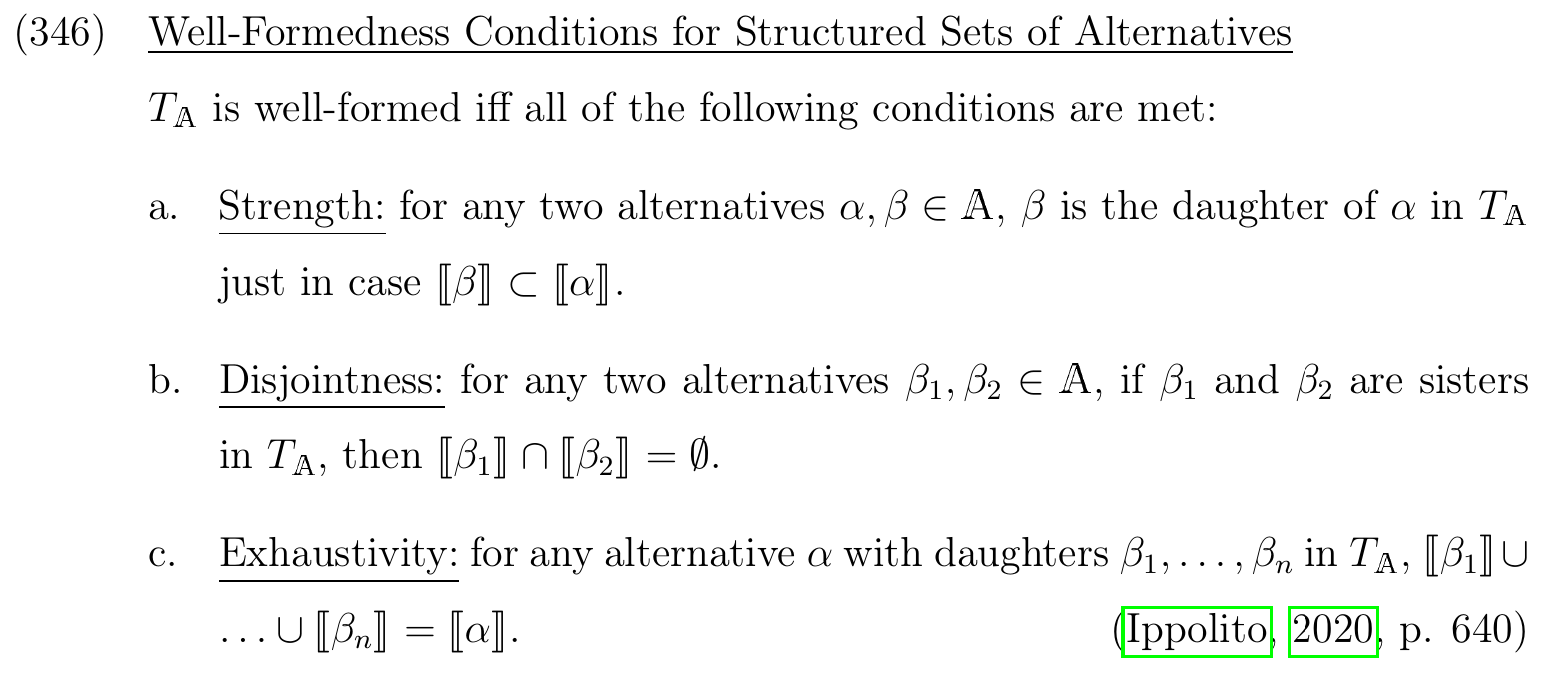
\includegraphics[width=0.8\textwidth]{graphics/ippolito-conditions.png}
\end{figure}\vfill
\end{frame}

\begin{frame}[t]
\subsectionpage\vskip 9pt\vfill
\begin{figure}
    \centering
    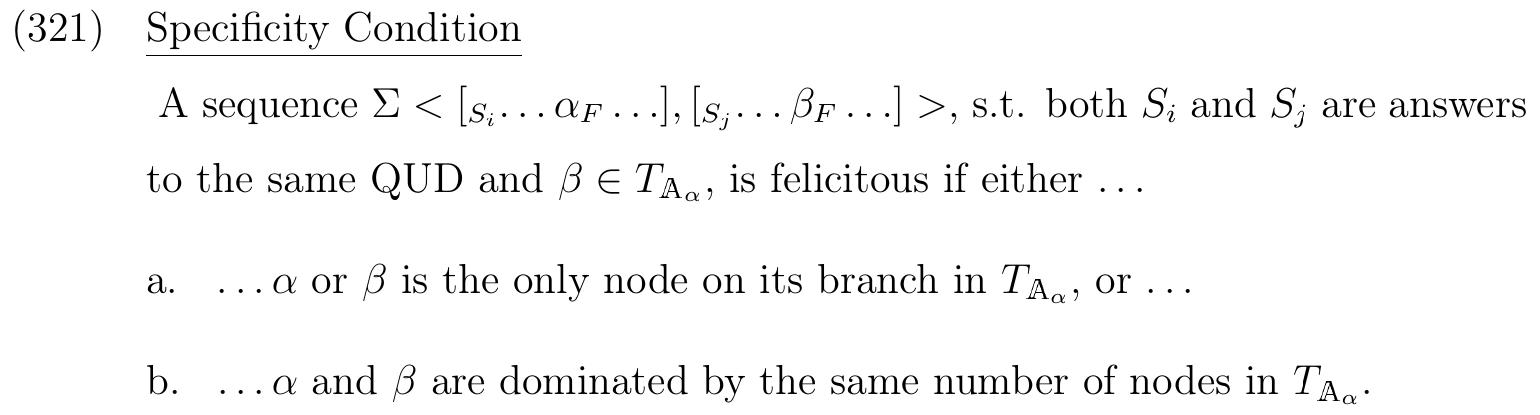
\includegraphics[width=0.8\textwidth]{graphics/ippolito-specificity.png}
\end{figure}\vfill
\end{frame}

\begin{frame}[t]
\subsectionpage\vskip 9pt\vfill
\begin{figure}
    \centering
    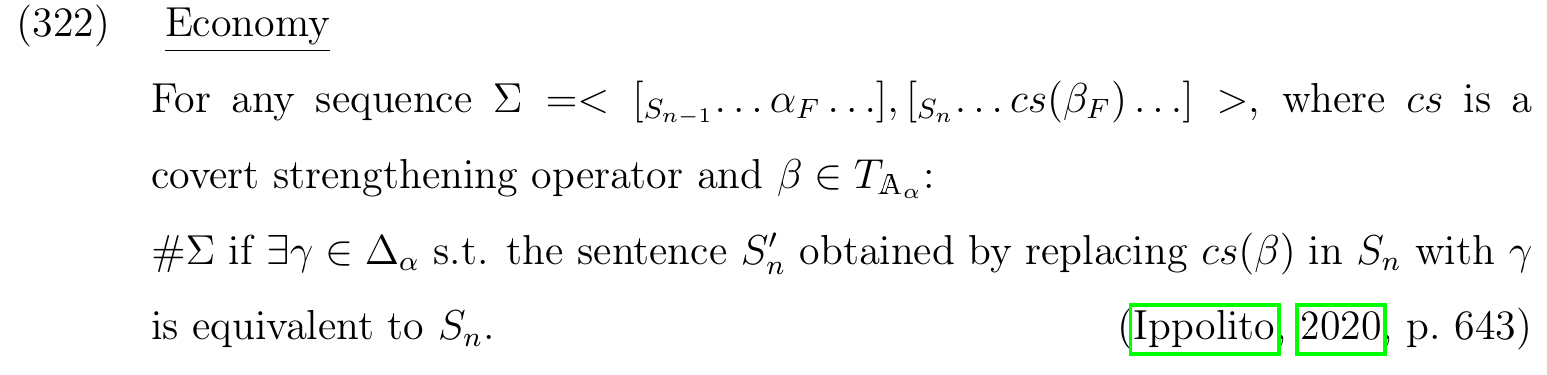
\includegraphics[width=0.8\textwidth]{graphics/ippolito-economy.png}
\end{figure}\vfill
\end{frame}

\begin{frame}[t]
\subsectionpage\vskip 9pt\vfill
\ex. John ate some or all of the cookies.

\ex. \#John ate all or some of the cookies.

\vfill
\begin{figure}
    \centering
    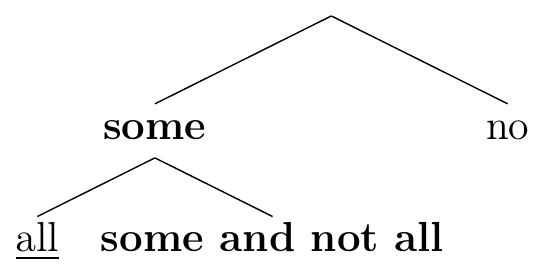
\includegraphics[width=0.3333\textwidth]{graphics/ippolito-someall-tree.png}
    \caption{Structured set of alternatives for some-but-not-all strenghtening.}
\end{figure}\vfill
\end{frame}

\begin{frame}[t]
\subsectionpage\vskip 9pt
\begin{itemize}
    \item World similarity relativised to focus value of conditional's antecedent
\end{itemize}\vfill
\begin{figure}
    \centering
    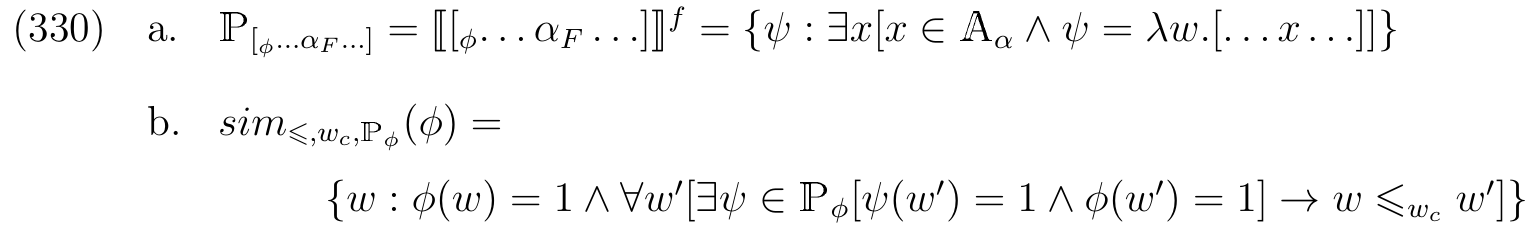
\includegraphics[width=0.8\textwidth]{graphics/ippolito-conditional-semantics.png}
\end{figure}\vfill
\end{frame}

\begin{frame}[t]
\subsectionpage\vskip 9pt\vfill
\begin{figure}
    \centering
    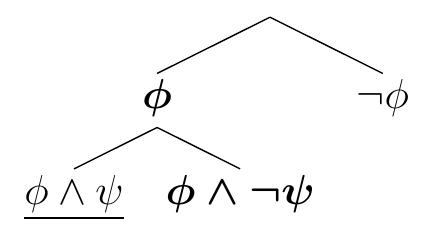
\includegraphics[width=0.3333\textwidth]{graphics/ippolito-general-rss-tree.png}
    \caption{Generalised structured set of alternatives for reverse Sobel sequences}
\end{figure}\vfill
\end{frame}

\begin{frame}[t]
\subsectionpage\vskip 9pt\vfill
\begin{figure}
    \centering
    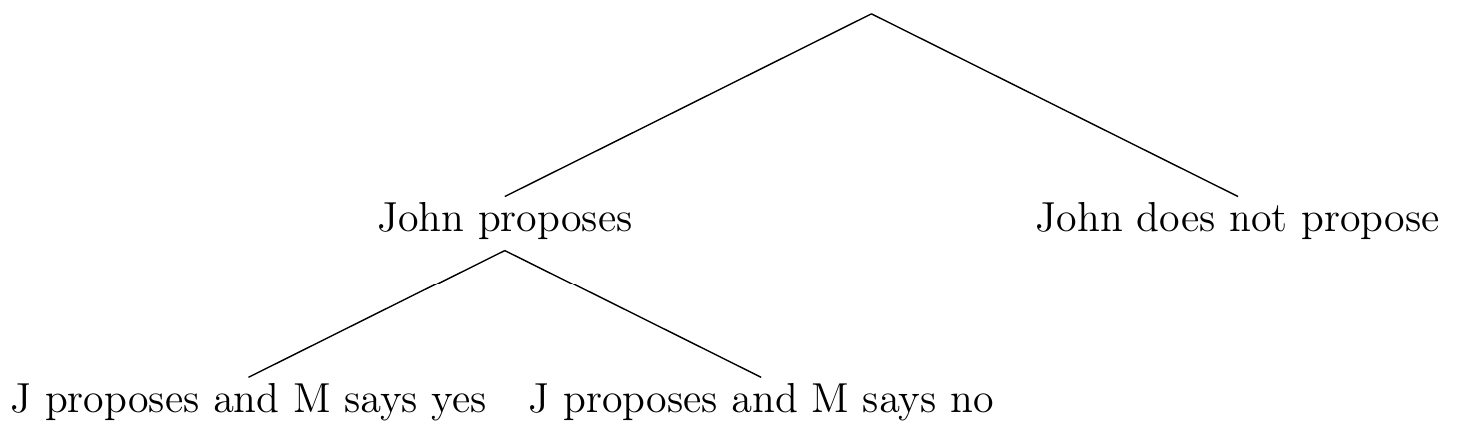
\includegraphics[width=0.9\textwidth]{graphics/ippolito-rss-prerestructure.png}
    \caption{Structured set of alternatives for $\phi\land\psi$-conditional}
\end{figure}\vfill
\end{frame}

\begin{frame}[t]
\subsectionpage\vskip 9pt\vfill
\begin{figure}
    \centering
    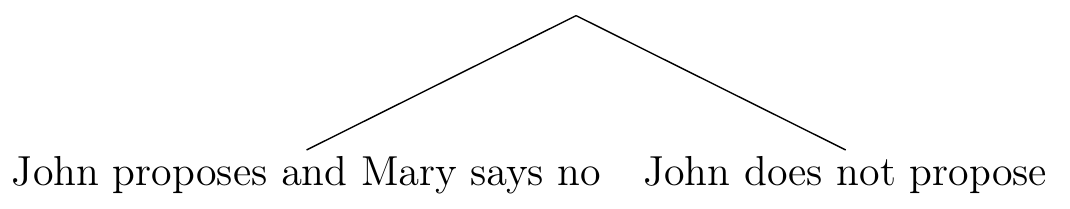
\includegraphics[width=0.6666\textwidth]{graphics/ippolito-rss-postrestructure.png}
    \caption{Restructured set of alternatives for $\phi$-conditional (epistemic exclusion)}
\end{figure}\vfill
\end{frame}

\begin{frame}[t]
\subsectionpage\vskip 9pt\vfill
\begin{figure}
    \centering
    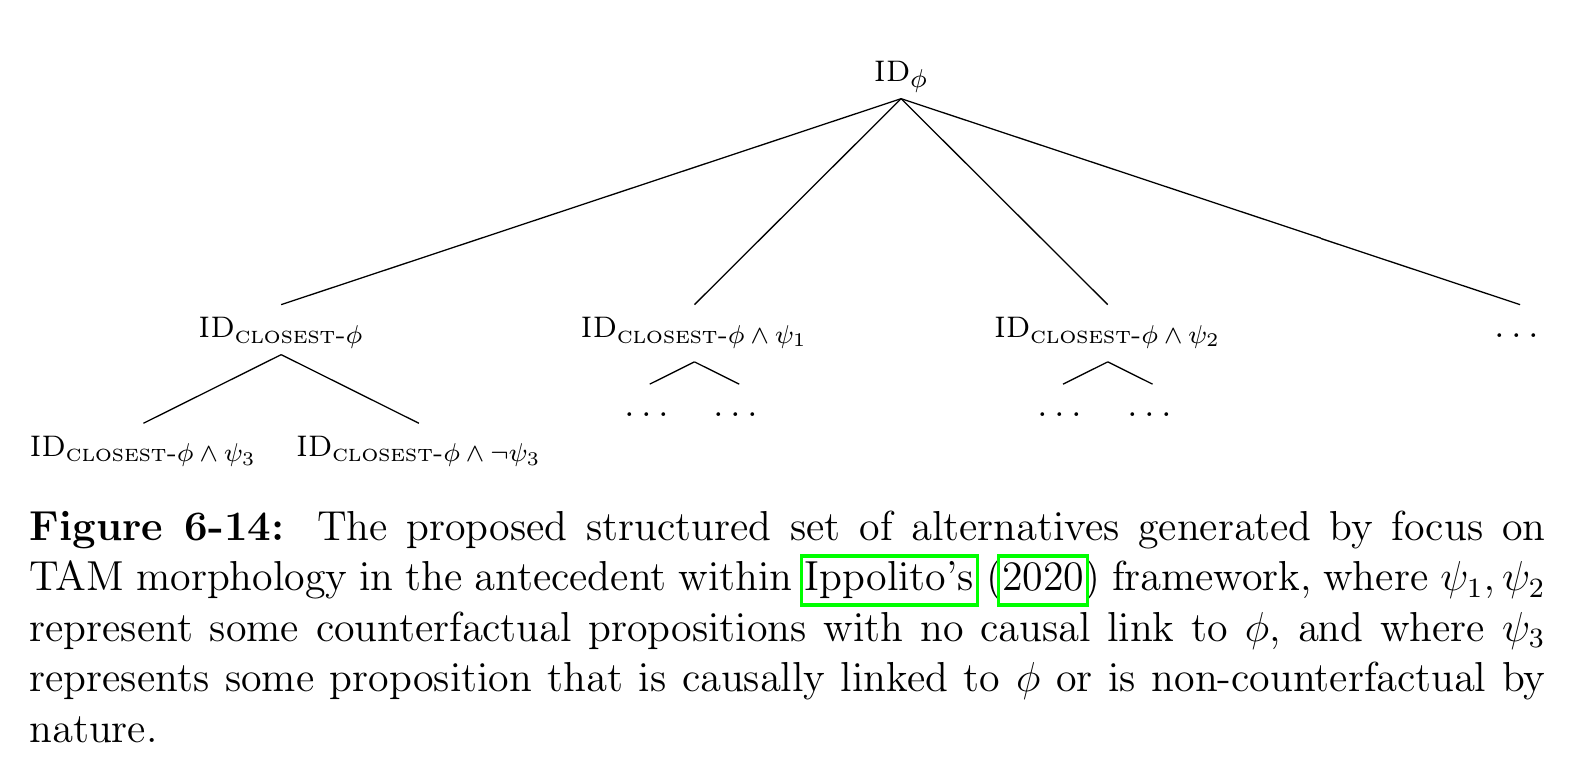
\includegraphics[trim=0 260 0 0,clip,width=0.9\textwidth]{graphics/ippolito-hybridtree.png}
    \caption{Structured set of alternatives for TAM-contrastive stress}
\end{figure}\vfill
\end{frame}

\subsection{\textit{Even}-Based NPIs}
\begin{frame}[t]
    \subsectionpage\vskip 9pt\vfill
\begin{figure}
    \centering
    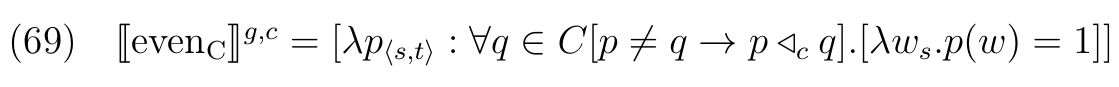
\includegraphics[width=0.7\textwidth]{graphics/crnic-even.png}
\end{figure}\vfill
\end{frame}

\begin{frame}[t]
    \subsectionpage\vskip 9pt\vfill
\begin{figure}
    \centering
    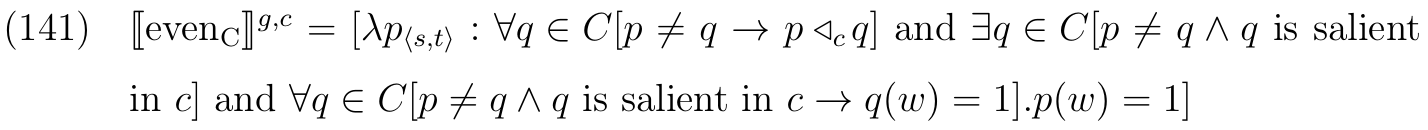
\includegraphics[width=0.8\textwidth]{graphics/crnic-even-extended.png}
\end{figure}\vfill
\end{frame}

\subsection{Crnic's SDM Context-Sensitivity}
\begin{frame}[t]
    \subsectionpage\vskip 9pt\vfill
\begin{figure}
    \centering
    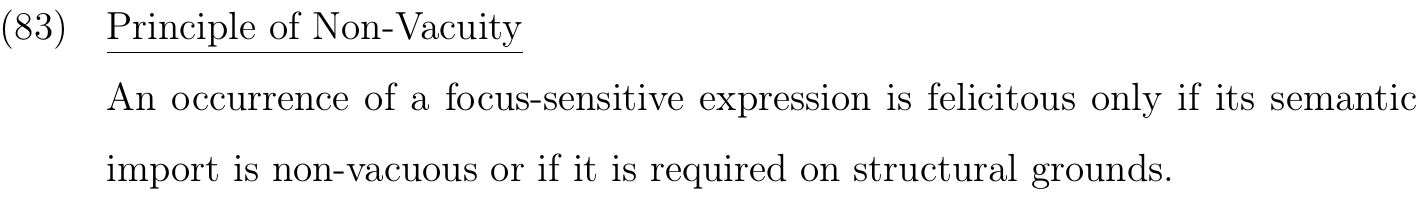
\includegraphics[width=0.8\textwidth]{graphics/crnic-nonvacuity.png}
\end{figure}\vfill
\end{frame}

\begin{frame}[t]
    \subsectionpage\vskip 9pt\vfill
\begin{figure}
    \centering
    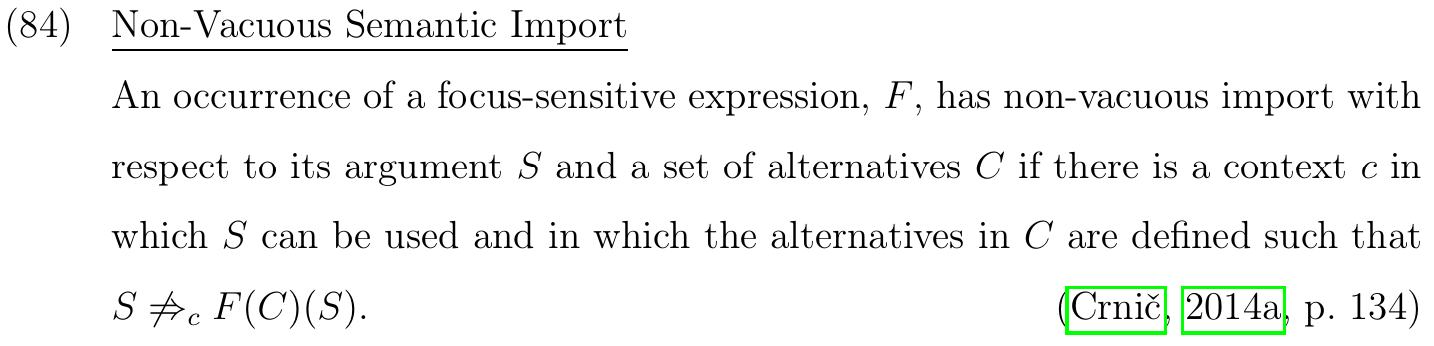
\includegraphics[width=0.8\textwidth]{graphics/crnic-semanticimport.png}
\end{figure}\vfill
\end{frame}

\begin{frame}[t]
    \subsectionpage\vskip 9pt\vfill
\begin{figure}
    \centering
    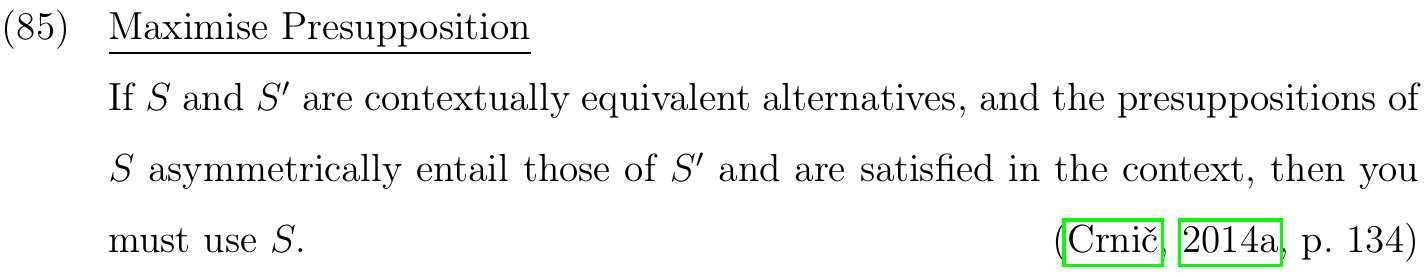
\includegraphics[width=0.8\textwidth]{graphics/crnic-maximisepresupposition.png}
\end{figure}\vfill
\end{frame}

\subsection{NPI Questions}
\begin{frame}[t]
    \subsectionpage\vskip 9pt\vfill
\begin{figure}
    \centering
    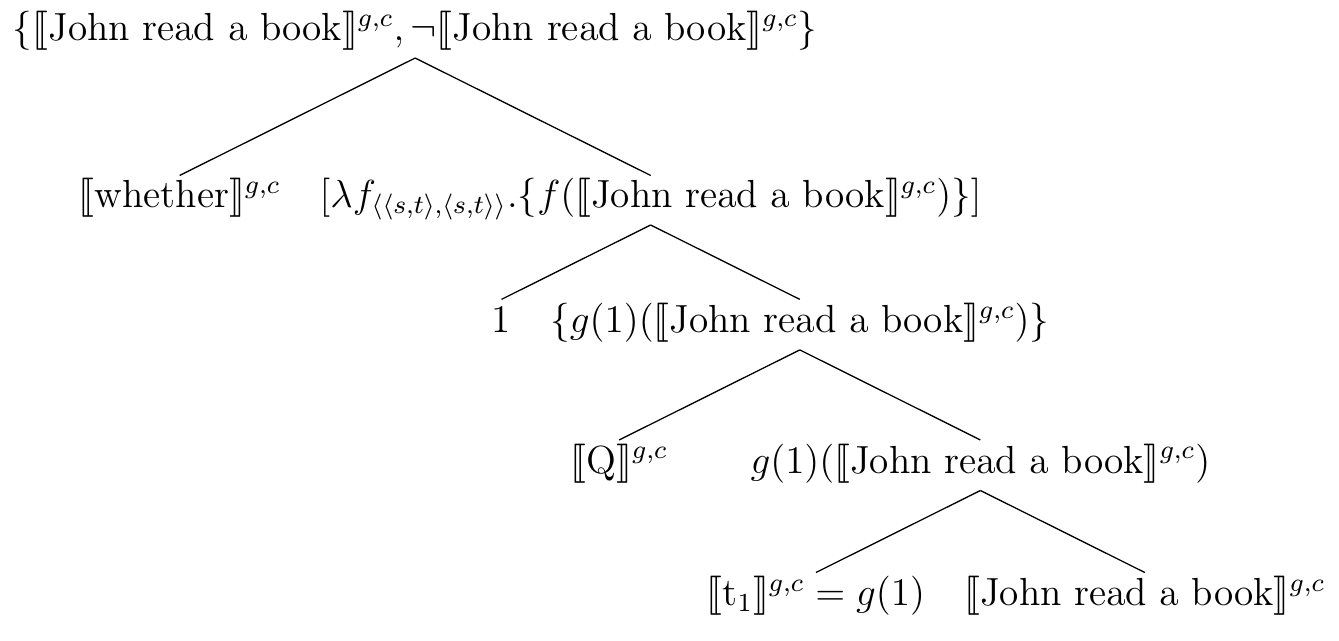
\includegraphics[height=8cm]{graphics/questions-guerzoni2003.png}
    \caption{Answers to Question Approach Tree}
\end{figure}\vfill
\end{frame}

\begin{frame}[t]
    \subsectionpage\vskip 9pt\vfill
\begin{figure}
    \centering
    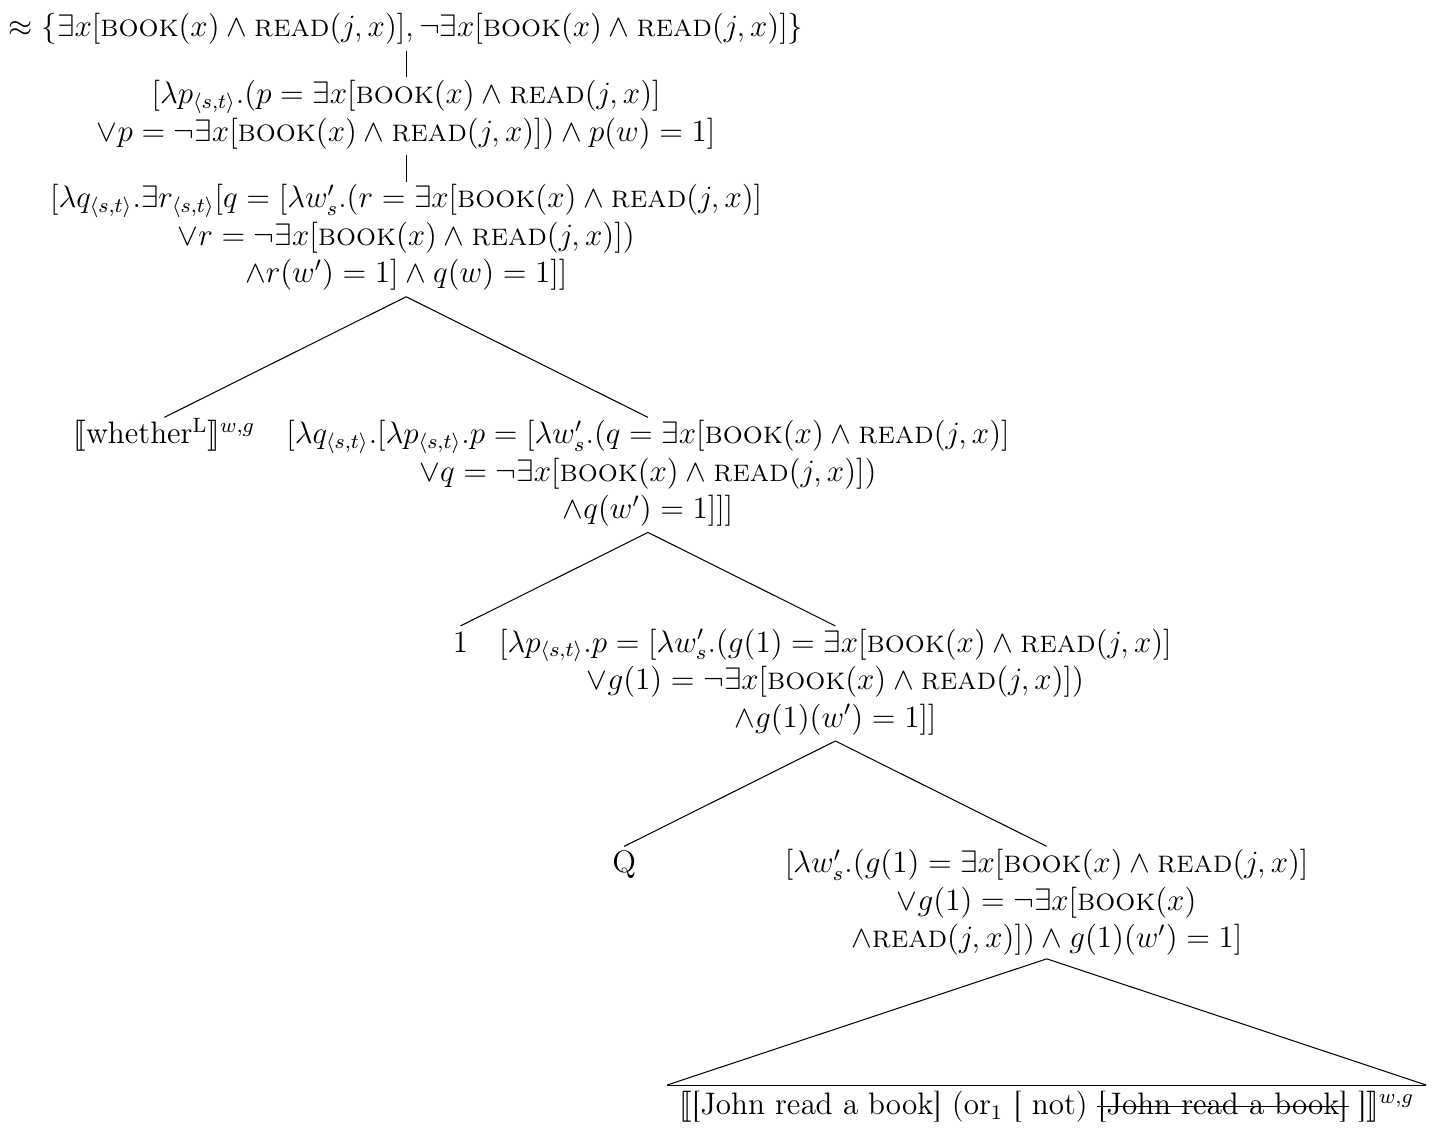
\includegraphics[height=8cm]{graphics/questions-guerzonisharvit2014.png}
    \caption{Environments in Questions Approach}
\end{figure}\vfill
\end{frame}
\end{document}
